\documentclass{article} % use larger type; default would be 10pt

\usepackage{pgfplots}
\usetikzlibrary{calc}
\usetikzlibrary{arrows}
\usetikzlibrary{patterns}
\usetikzlibrary{calc,intersections,through,backgrounds}
\usetikzlibrary{decorations.pathreplacing}
        \newcommand\degree[0]{^{\circ}}
        \newcommand\abs[1]{\left|#1\right|}

\title{Play with TikZ}
\author{Just Us}
%\date{} % Activate to display a given date or no date (if empty),
         % otherwise the current date is printed 

\begin{document}
\maketitle


\section{Chap 2 Section 3}



fig-2-3-ex1 line


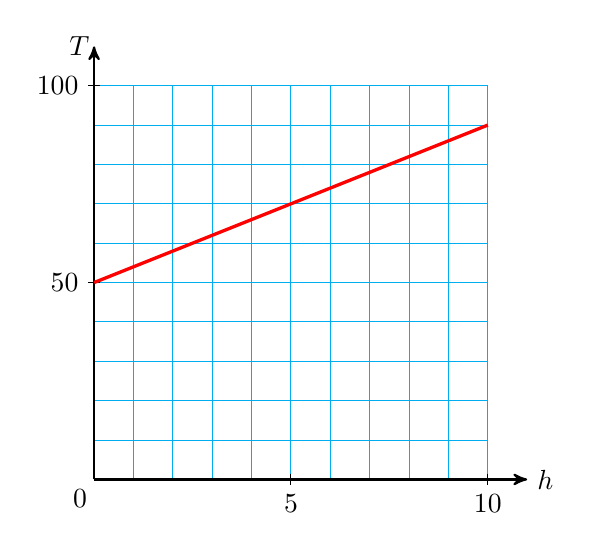
\begin{tikzpicture} [scale=0.5]
\coordinate (O) at (0,0);
\draw[cyan] (O) grid (10,10);
\draw[black,thick, ->, >=stealth'] (O)--(11,0) node[right]{$h$};
\draw[black,thick, ->, >=stealth'] (O)--(0,11) node[left, xshift=2]{$T$};
\foreach \x in  {5,10} {
 \draw[black] (\x,.15) --++(0,-.3)  node[below]   {\x};
}
\foreach \y [evaluate=\y as \yi using int( 10* \y )] in  {5,10} {
 \draw[black] (.15,\y) --++(-.3,0)  node[left]   {\yi};
}
\draw [red, very thick]  (0,5) -- (10,9);
\node[below left, xshift=1] at (O) {0};
\end{tikzpicture}
\newline



fig-2-3-1 5-by-5 grid

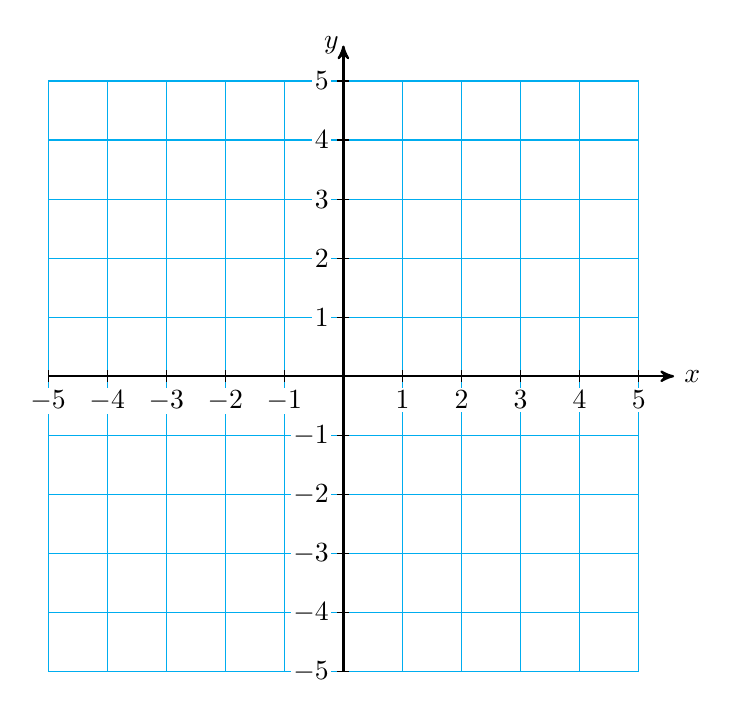
\begin{tikzpicture} [scale=.75]
\coordinate (O) at (0,0);
\draw[cyan] (-5,-5) grid (5,5);
\draw[black,thick, ->, >=stealth'] (-5,0)--(5.6,0) node[right]{$x$};
\draw[black,thick, ->, >=stealth'] (0,-5)--(0,5.6) node[left, xshift=2]{$y$};
\foreach \x in  {-5,-4, ...,-1, 1, 2, ...,5} {
 \draw[black] (\x,.1) --++(0,-.2)  node[below, yshift=-2, fill=white, inner sep=1]   {$\x$};
 \draw[black] (.1,\x) --++(-.2,0)  node[left, xshift=-2, fill=white, inner sep=1]   {$\x$};
}
\end{tikzpicture}
\newline


fig-2-3-ex2 points on 5-by-5 grid

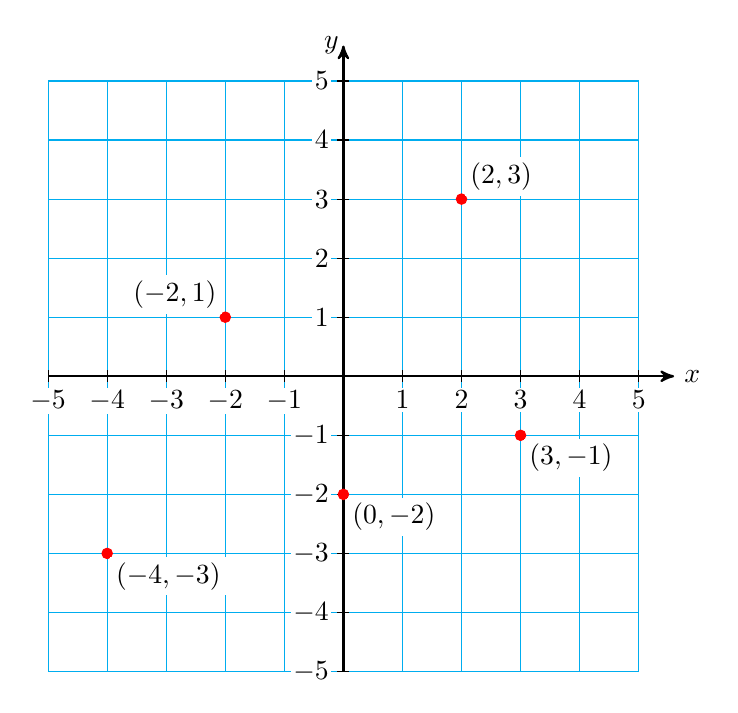
\begin{tikzpicture} [scale=.75]
\coordinate (O) at (0,0);
\draw[cyan] (-5,-5) grid (5,5);
\draw[black,thick, ->, >=stealth'] (-5,0)--(5.6,0) node[right]{$x$};
\draw[black,thick, ->, >=stealth'] (0,-5)--(0,5.6) node[left, xshift=2]{$y$};
\foreach \x in  {-5,-4, ...,-1, 1, 2, ...,5} {
 \draw[black] (\x,.1) --++(0,-.2)  node[below, yshift=-2, fill=white, inner sep=1]   {$\x$};
 \draw[black] (.1,\x) --++(-.2,0)  node[left, xshift=-2, fill=white, inner sep=1]   {$\x$};
}
\filldraw[red] (2,3) circle (2.5pt) node[fill=white, text=black, inner sep=2, above right, xshift=1, yshift=1] {$(2,3)$};
\filldraw[red] (-2,1) circle (2.5pt) node[fill=white, text=black, inner sep=2, above left, xshift=-1, yshift=1] {$(-2,1)$};
\filldraw[red] (-4,-3) circle (2.5pt) node[fill=white, text=black, inner sep=2, below right, xshift=1, yshift=-1] {$(-4,-3)$};
\filldraw[red] (0,-2) circle (2.5pt) node[fill=white, text=black, inner sep=2, below right, xshift=1, yshift=-1] {$(0,-2)$};
\filldraw[red] (3,-1) circle (2.5pt) node[fill=white, text=black, inner sep=2, below right, xshift=1, yshift=-1] {$(3,-1)$};
\end{tikzpicture}
\newline


fig-2-3-ex4a line


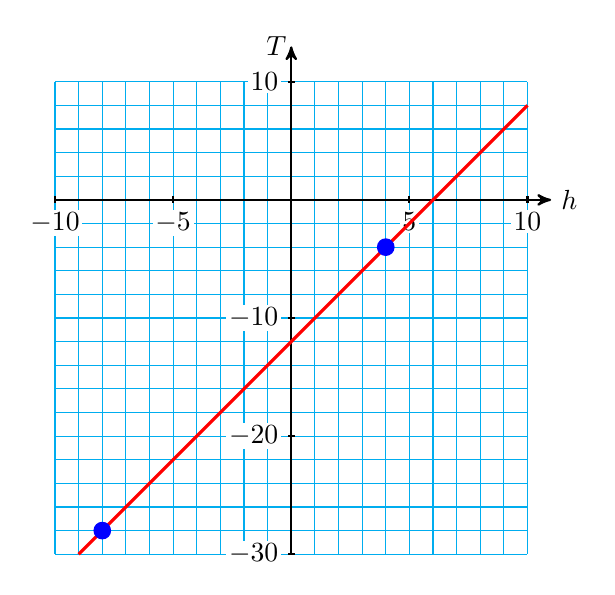
\begin{tikzpicture} [xscale=0.3, yscale=0.15]
\draw[cyan] (-10,-30) grid[ystep=2] (10,10);
\draw[black,thick, ->, >=stealth'] (-10,0)--(11,0) node[right]{$h$};
\draw[black,thick, ->, >=stealth'] (0,-30)--(0,13) node[left, xshift=2]{$T$};
\foreach \x in  {-10,-5,5,10} {
 \draw[black, thick] (\x,.3) --++(0,-.6)  node[below, yshift=-2, fill=white, inner sep=1]   {$\x$};
}
\foreach \y  in  {-30,-20,-10,10} {
 \draw[black,thick] (.15,\y) --++(-.3,0)  node[left, xshift=-2, fill=white, inner sep=1]   {$\y$};
}
\draw [red, very thick]  (-9,-30) -- (10,8);
\filldraw[blue] (-8,-28) ellipse (.35cm and .7cm);
\filldraw[blue] (4,-4) ellipse (.35cm and .7cm);
\end{tikzpicture}
\newline


fig-2-3-ex4a line


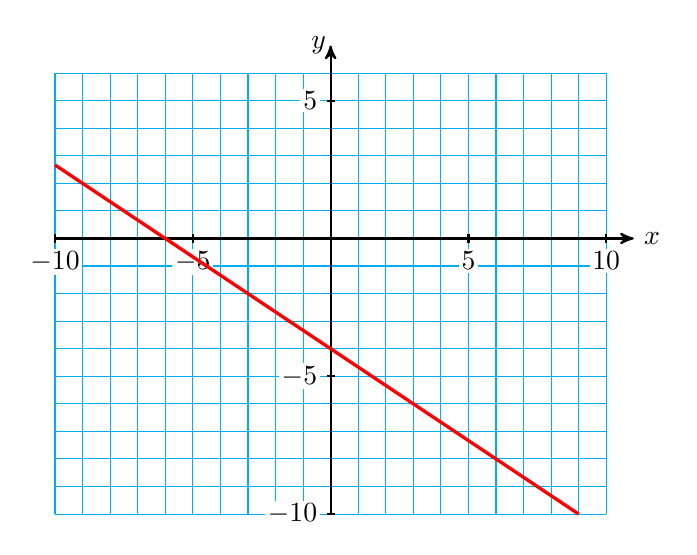
\begin{tikzpicture} [scale=0.35]
\draw[cyan] (-10,-10) grid (10,6);
\draw[black,thick, ->, >=stealth'] (-10,0)--(11,0) node[right]{$x$};
\draw[black,thick, ->, >=stealth'] (0,-10)--(0,7) node[left, xshift=2]{$y$};
\foreach \x in  {-10,-5,5,10} {
 \draw[black, thick] (\x,.15) --++(0,-.3)  node[below, yshift=-2, fill=white, inner sep=1]   {$\x$};
}
\foreach \y  in  {-10,-5,5} {
 \draw[black,thick] (.15,\y) --++(-.3,0)  node[left, xshift=-2, fill=white, inner sep=1]   {$\y$};
}
\draw [red, very thick]  (-10,8/3) -- (9,-10);
\end{tikzpicture}
\newline


fig-2-3-ex4b line and point


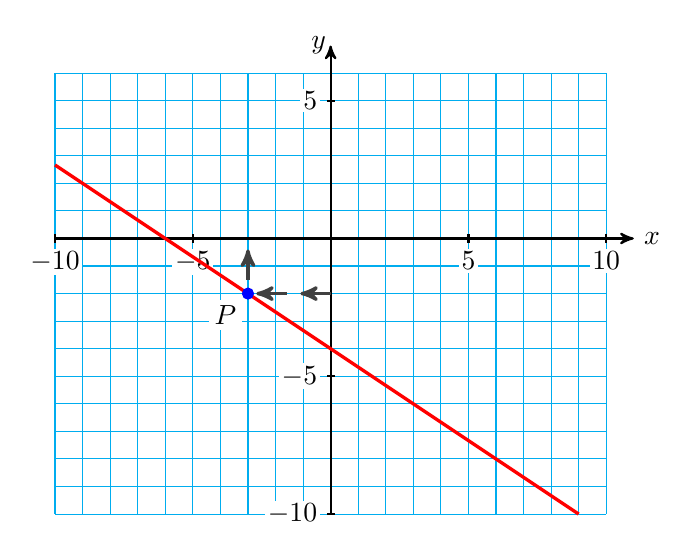
\begin{tikzpicture} [scale=0.35]
\draw[cyan] (-10,-10) grid (10,6);
\draw[black,thick, ->, >=stealth'] (-10,0)--(11,0) node[right]{$x$};
\draw[black,thick, ->, >=stealth'] (0,-10)--(0,7) node[left, xshift=2]{$y$};
\foreach \x in  {-10,-5,5,10} {
 \draw[black, thick] (\x,.15) --++(0,-.3)  node[below, yshift=-2, fill=white, inner sep=1]   {$\x$};
}
\foreach \y  in  {-10,-5,5} {
 \draw[black,thick] (.15,\y) --++(-.3,0)  node[left, xshift=-2, fill=white, inner sep=1]   {$\y$};
}
\draw [red, very thick]  (-10,8/3) -- (9,-10);
\coordinate (P) at (-3,-2);
\foreach \x in {0,-1.6}
 \draw[darkgray,very thick, ->, >=stealth'] (\x,-2)--++(-1.1,0);
\draw[darkgray,very thick, ->, >=stealth'] (-3,-1.5)--++(0,1.1);
\filldraw[blue]  (P) circle (2mm) node[below left, xshift=-2, yshift=-2, text=black, fill=white, inner sep=2] {$P$};
\end{tikzpicture}
\newline





hp-2-3-1 6-by-6 grid

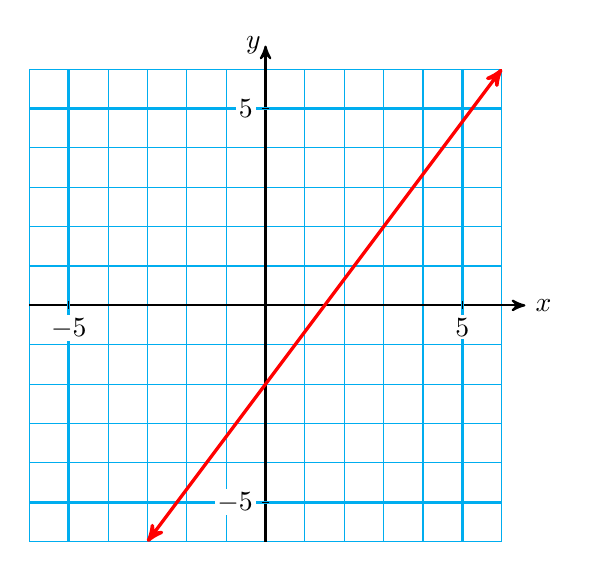
\begin{tikzpicture} [scale=.5]
\coordinate (O) at (0,0);
\draw[cyan] (-6,-6) grid (6,6);
\draw[black,thick, ->, >=stealth'] (-6,0)--(6.6,0) node[right]{$x$};
\draw[black,thick, ->, >=stealth'] (0,-6)--(0,6.6) node[left, xshift=2]{$y$};
\foreach \x in  {-5, 5} {
 \draw[cyan, very thick] (\x,-6) --++(0,12);
 \draw[cyan, very thick] (-6,\x) --++(12,0);
 \draw[black] (\x,.1) --++(0,-.2)  node[below, yshift=-2, fill=white, inner sep=1]   {$\x$};
 \draw[black] (.1,\x) --++(-.2,0)  node[left, xshift=-2, fill=white, inner sep=1]   {$\x$};
}
\draw[red, very thick, <->, >=stealth'] (-3,-6)--(6,6);
\end{tikzpicture}
\newline



hp-2-3-2 6-by-6 grid

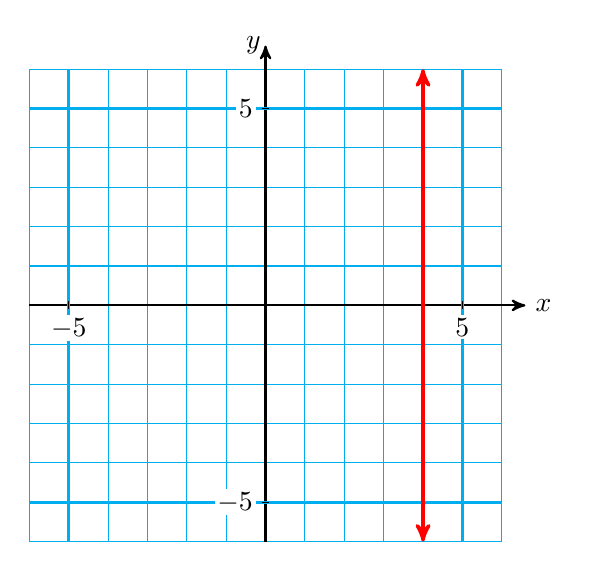
\begin{tikzpicture} [scale=.5]
\coordinate (O) at (0,0);
\draw[cyan] (-6,-6) grid (6,6);
\draw[black,thick, ->, >=stealth'] (-6,0)--(6.6,0) node[right]{$x$};
\draw[black,thick, ->, >=stealth'] (0,-6)--(0,6.6) node[left, xshift=2]{$y$};
\foreach \x in  {-5, 5} {
 \draw[cyan, very thick] (\x,-6) --++(0,12);
 \draw[cyan, very thick] (-6,\x) --++(12,0);
 \draw[black] (\x,.1) --++(0,-.2)  node[below, yshift=-2, fill=white, inner sep=1]   {$\x$};
 \draw[black] (.1,\x) --++(-.2,0)  node[left, xshift=-2, fill=white, inner sep=1]   {$\x$};
}
\draw[red, very thick, <->, >=stealth'] (4,-6)--(4,6);
\end{tikzpicture}
\newline



hp-2-3-3 points in plane

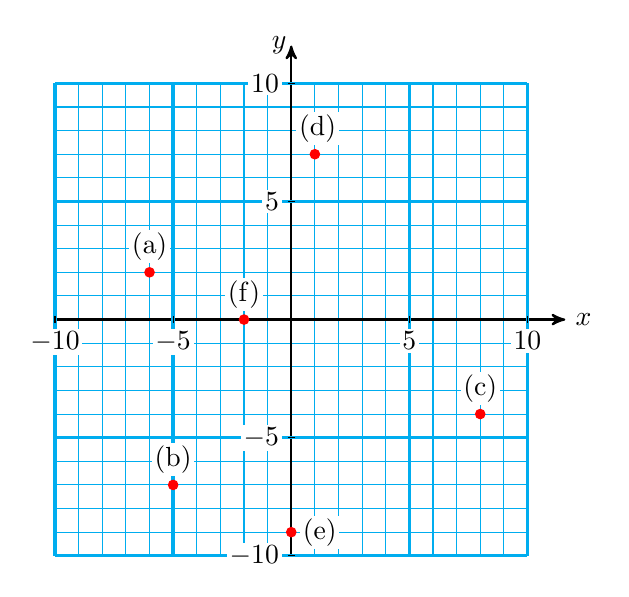
\begin{tikzpicture} [scale=.3]
\coordinate (O) at (0,0);
\draw[cyan] (-10,-10) grid (10,10);
\draw[black,thick, ->, >=stealth'] (-10,0)--(11.6,0) node[right]{$x$};
\draw[black,thick, ->, >=stealth'] (0,-10)--(0,11.6) node[left, xshift=2]{$y$};
\foreach \x in  {-5, 5, -10, 10} {
 \draw[cyan, very thick] (\x,-10) --++(0,20);
 \draw[cyan, very thick] (-10,\x) --++(20,0);
 \draw[black] (\x,.15) --++(0,-.3)  node[below, yshift=-2, fill=white, inner sep=1]   {$\x$};
 \draw[black] (.15,\x) --++(-.3,0)  node[left, xshift=-2, fill=white, inner sep=1]   {$\x$};
}
\filldraw[red]  (-6,2) circle (2mm) node[above, yshift=3, fill=white, inner sep=1, text=black] {(a)}; 
\filldraw[red]  (-5,-7) circle (2mm) node[above, yshift=3, fill=white, inner sep=1, text=black] {(b)}; 
\filldraw[red]  (8,-4) circle (2mm) node[above, yshift=3, fill=white, inner sep=1, text=black] {(c)}; 
\filldraw[red]  (1,7) circle (2mm) node[above, xshift=1, yshift=3, fill=white, inner sep=1, text=black] {(d)}; 
\filldraw[red]  (0,-9) circle (2mm) node[right, xshift=3, fill=white, inner sep=1, text=black] {(e)}; 
\filldraw[red]  (-2,0) circle (2mm) node[above, yshift=3, fill=white, inner sep=1, text=black] {(f)}; 
\end{tikzpicture}
\newline



hp-2-3-4 points in plane

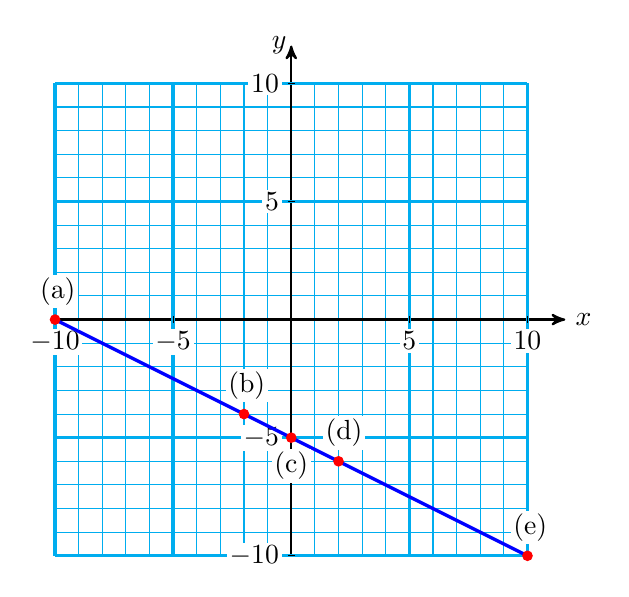
\begin{tikzpicture} [scale=.3]
\coordinate (O) at (0,0);
\draw[cyan] (-10,-10) grid (10,10);
\draw[black,thick, ->, >=stealth'] (-10,0)--(11.6,0) node[right]{$x$};
\draw[black,thick, ->, >=stealth'] (0,-10)--(0,11.6) node[left, xshift=2]{$y$};
\foreach \x in  {-5, 5, -10, 10} {
 \draw[cyan, very thick] (\x,-10) --++(0,20);
 \draw[cyan, very thick] (-10,\x) --++(20,0);
 \draw[black] (\x,.15) --++(0,-.3)  node[below, yshift=-2, fill=white, inner sep=1]   {$\x$};
 \draw[black] (.15,\x) --++(-.3,0)  node[left, xshift=-2, fill=white, inner sep=1]   {$\x$};
}
\draw[blue, very thick] (-10,0)--(10,-10);
\filldraw[red]  (-10,0) circle (2mm) node[above, xshift=1, yshift=4, fill=white, inner sep=1, text=black] {(a)}; 
\filldraw[red]  (-2,-4) circle (2mm) node[above, xshift=1, yshift=4, fill=white, inner sep=1, text=black] {(b)}; 
\filldraw[red]  (0,-5) circle (2mm) node[below, yshift=-4, fill=white, inner sep=1, text=black] {(c)}; 
\filldraw[red]  (2,-6) circle (2mm) node[above, xshift=2, yshift=4, fill=white, inner sep=1, text=black] {(d)}; 
\filldraw[red]  (10,-10) circle (2mm) node[above, xshift=1, yshift=4, fill=white, inner sep=1, text=black] {(e)}; 
 \end{tikzpicture}
\newline



hp-2-3-5 points in plane

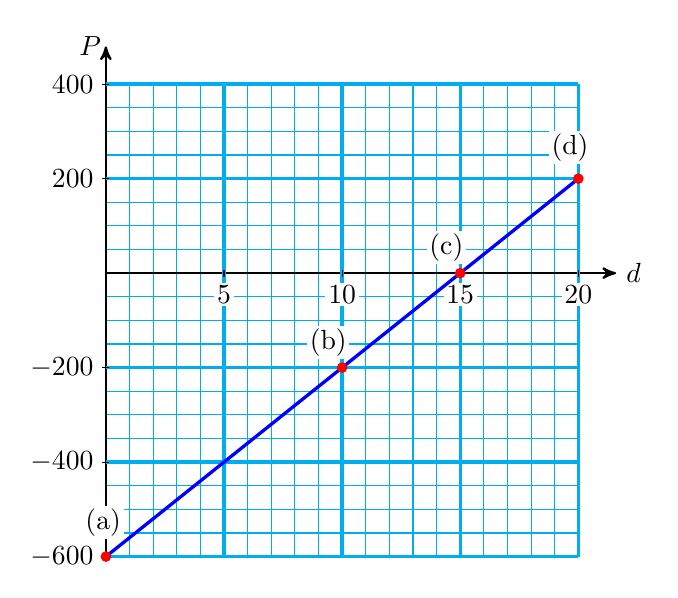
\begin{tikzpicture} [scale=.3]
\coordinate (O) at (0,0);
\draw[cyan] (0,-12) grid (20,8);
\draw[black,thick, ->, >=stealth'] (0,0)--(21.6,0) node[right]{$d$};
\draw[black,thick, ->, >=stealth'] (0,-12)--(0,9.6) node[left, xshift=2]{$P$};
\foreach \x in  {5, 10, 15, 20} {
 \draw[cyan, very thick] (\x,-12) --++(0,20);
 \draw[black] (\x,.15) --++(0,-.3)  node[below, yshift=-2, fill=white, inner sep=1]   {$\x$};
}
\foreach \y [evaluate=\y as \yi using int( 50* \y )] in {-12, -8, -4, 4, 8} {
 \draw[cyan, very thick] (0,\y) --++(20,0);
 \draw[black] (.15,\y) --++(-.3,0)  node[left, xshift=-2, fill=white, inner sep=1]   {$\yi$};
}
\draw[blue, very thick] (0,-12)--(20,4);
\filldraw[red]  (0,-12) circle (2mm) node[above, xshift=-1, yshift=6, fill=white, inner sep=1, text=black] {(a)}; 
\filldraw[red]  (10,-4) circle (2mm) node[above, xshift=-5, yshift=3, fill=white, inner sep=1, text=black] {(b)}; 
\filldraw[red]  (15,0) circle (2mm) node[above, xshift=-5, yshift=3, fill=white, inner sep=1, text=black] {(c)}; 
\filldraw[red]  (20,4) circle (2mm) node[above, xshift=-3, yshift=5, fill=white, inner sep=1, text=black] {(d)}; 
\end{tikzpicture}
\newline



hp-2-3-6 grid

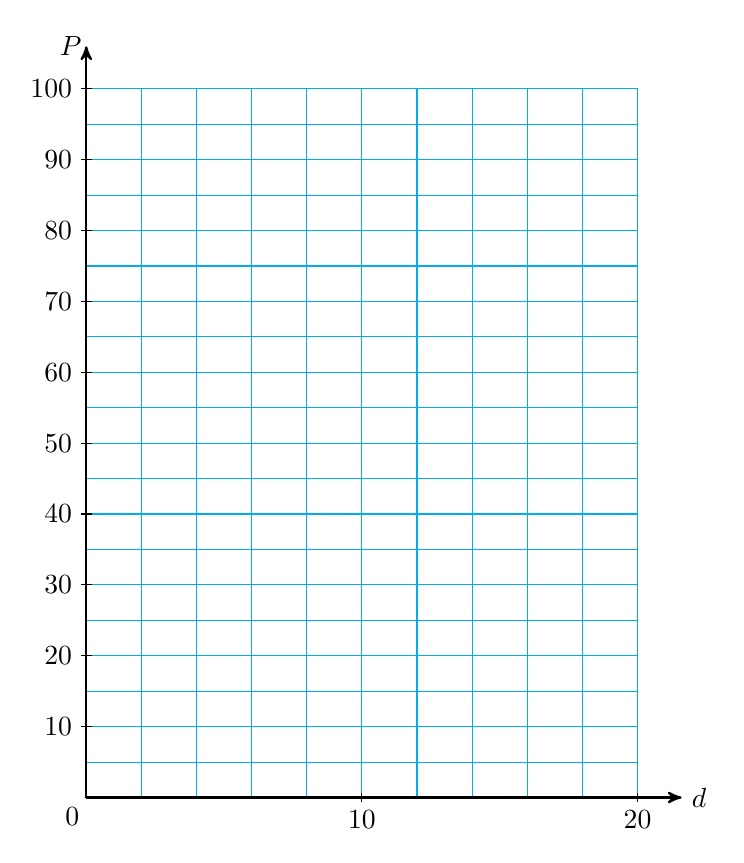
\begin{tikzpicture} [xscale=.35, yscale=.09]
\coordinate (O) at (0,0);
\draw[cyan] (O) grid[xstep=2, ystep=5] (20,100);
\draw[black,thick, ->, >=stealth'] (O)--(21.6,0) node[right]{$d$};
\draw[black,thick, ->, >=stealth'] (O)--(0,106) node[left, xshift=2]{$P$};
\foreach \x in  {10,20} {
 \draw[black] (\x,.6) --++(0,-1.2)  node[below, yshift=-2, fill=white, inner sep=1]   {$\x$};
}
\foreach \x in  {10,20,...,100} {
 \draw[black] (.2,\x) --++(-.4,0)  node[left, xshift=-2, fill=white, inner sep=1]   {$\x$};
}
\node[below left, xshift=1] at (O) {0};
\end{tikzpicture}
\newline



hp-2-3-7 grid

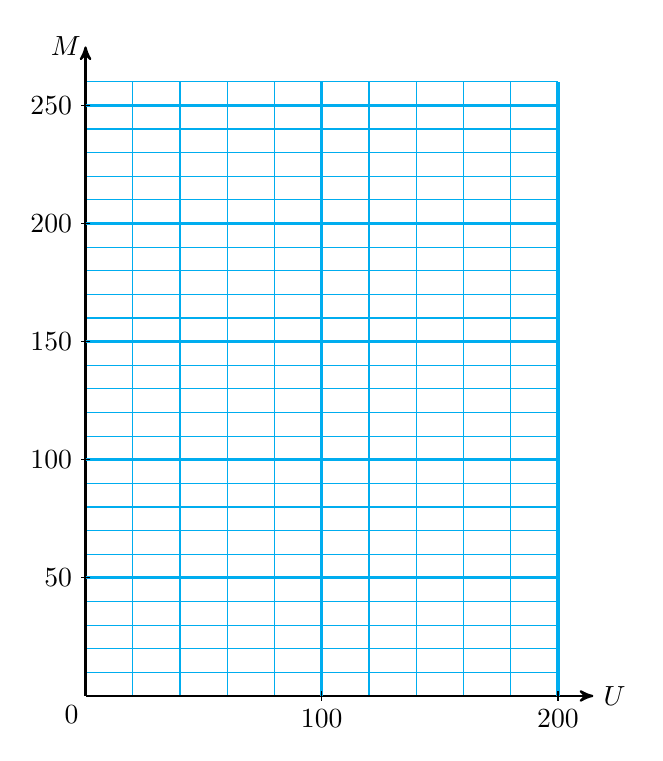
\begin{tikzpicture} [scale=.03]
\coordinate (O) at (0,0);
\draw[cyan] (O) grid[xstep=20, ystep=10] (200,260);
\draw[black,thick, ->, >=stealth'] (O)--(215,0) node[right]{$U$};
\draw[black,thick, ->, >=stealth'] (O)--(0,275) node[left, xshift=2]{$M$};
\foreach \x in  {100,200} {
 \draw[cyan,very thick] (\x,0) --++(0,260); 
 \draw[black] (\x,2) --++(0,-4)  node[below, yshift=-2, fill=white, inner sep=1]   {$\x$};
}
\foreach \x in  {50,100,...,250} {
 \draw[cyan, very thick] (0,\x) --++(200,0); 
 \draw[black] (2,\x) --++(-4,0)  node[left, xshift=-2, fill=white, inner sep=1]   {$\x$};
}
\node[below left, xshift=1] at (O) {0};
\end{tikzpicture}
\newline



hp-2-3-7ans grid

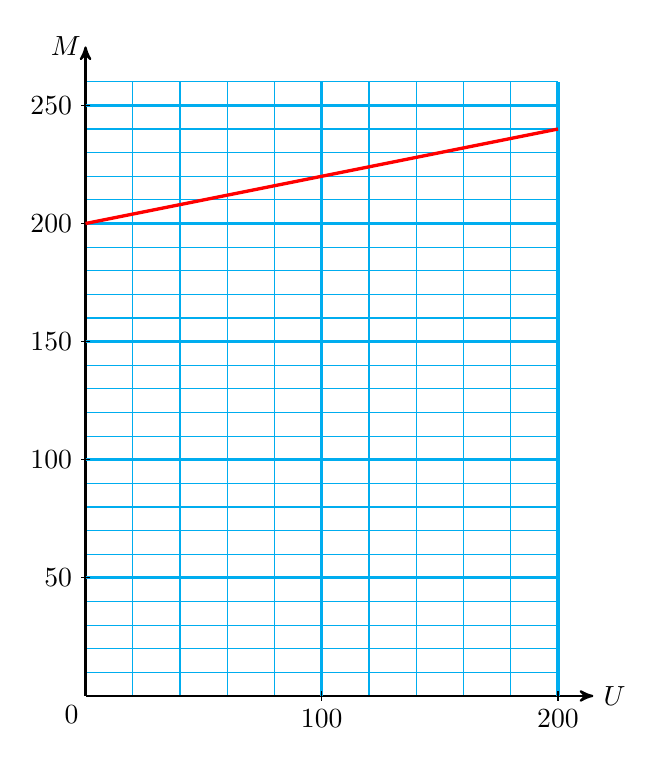
\begin{tikzpicture} [scale=.03]
\coordinate (O) at (0,0);
\draw[cyan] (O) grid[xstep=20, ystep=10] (200,260);
\draw[black,thick, ->, >=stealth'] (O)--(215,0) node[right]{$U$};
\draw[black,thick, ->, >=stealth'] (O)--(0,275) node[left, xshift=2]{$M$};
\foreach \x in  {100,200} {
 \draw[cyan,very thick] (\x,0) --++(0,260); 
 \draw[black] (\x,2) --++(0,-4)  node[below, yshift=-2, fill=white, inner sep=1]   {$\x$};
}
\foreach \x in  {50,100,...,250} {
 \draw[cyan, very thick] (0,\x) --++(200,0); 
 \draw[black] (2,\x) --++(-4,0)  node[left, xshift=-2, fill=white, inner sep=1]   {$\x$};
}
\node[below left, xshift=1] at (O) {0};
\draw[red, very thick] (0,200)--(200,240);
%\foreach \x in {20,40,80,100,200} 
%\filldraw[blue] (\x, {200+\x/5}) circle (2.5cm);
\end{tikzpicture}
\newline



hp-2-3-8 grid

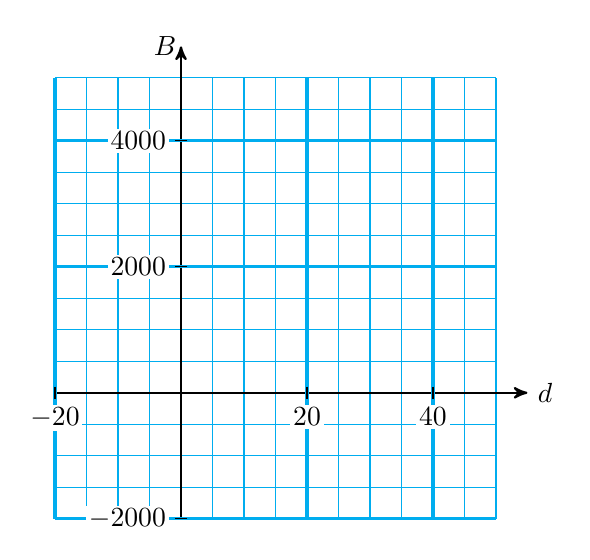
\begin{tikzpicture} [scale=.4]
\draw[cyan] (-4,-4) grid(10,10);
\draw[black,thick, ->, >=stealth'] (-4,0)--(11,0) node[right]{$d$};
\draw[black,thick, ->, >=stealth'] (0,-4)--(0,11) node[left, xshift=2]{$B$};
\foreach \x [evaluate=\x as \xi using int( 5* \x )] in  {-4,4,8} {
 \draw[cyan,very thick] (\x,-4) --(\x,10); 
 \draw[black] (\x,.2) --++(0,-.4)  node[below, yshift=-2, fill=white, inner sep=1]   {$\xi$};
}
\foreach \x [evaluate=\x as \xi using int( 500* \x )] in  {-4,4,8} {
 \draw[cyan, very thick] (-4,\x) --(10,\x); 
 \draw[black] (.2,\x) --++(-.4,0)  node[left, xshift=-2, fill=white, inner sep=1]   {$\xi$};
}
\end{tikzpicture}
\newline



hp-2-3-9 line on grid

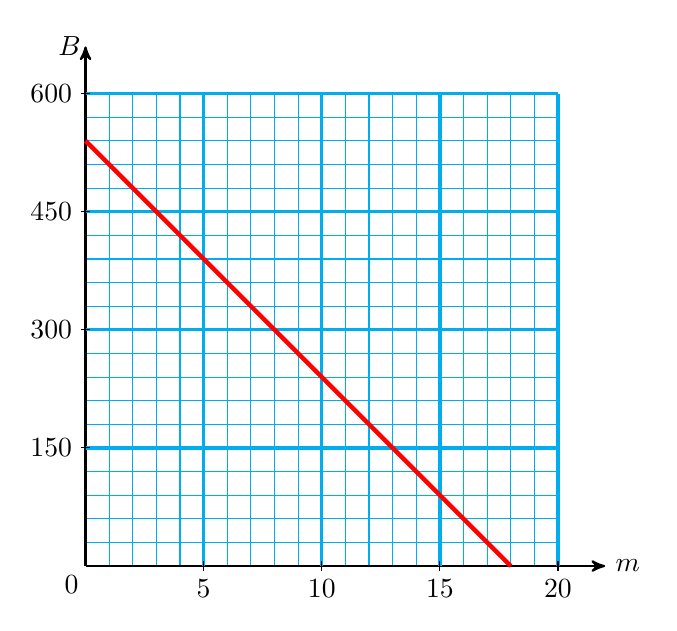
\begin{tikzpicture} [scale=.3]
\coordinate (O) at (0,0);
\draw[cyan] (O) grid(20,20);
\draw[black,thick, ->, >=stealth'] (O)--(22,0) node[right]{$m$};
\draw[black,thick, ->, >=stealth'] (O)--(0,22) node[left, xshift=2]{$B$};
\foreach \x in  {5,10,15, 20} {
 \draw[cyan,very thick] (\x,0) --(\x,20); 
 \draw[black] (\x,.2) --++(0,-.4)  node[below, yshift=-2, fill=white, inner sep=1]   {$\x$};
}
\foreach \x [evaluate=\x as \xi using int( 30* \x )] in  {5,10,15, 20} {
 \draw[cyan, very thick] (0,\x) --(20,\x); 
 \draw[black] (.2,\x) --++(-.4,0)  node[left, xshift=-2, fill=white, inner sep=1]   {$\xi$};
}
\draw[red, ultra thick] (0,18)--(18,0);
\node[below left, xshift=1] at (O) {0};
\end{tikzpicture}
\newline



hp-2-3-10  grid

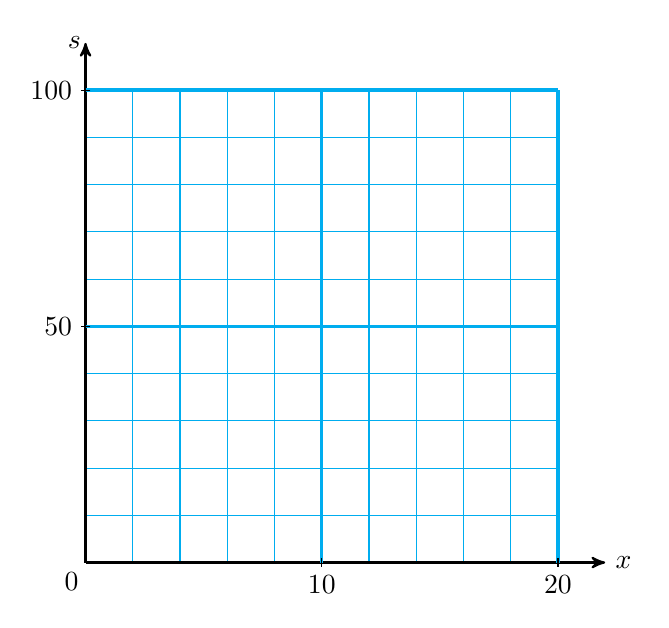
\begin{tikzpicture} [scale=.30]
\coordinate (O) at (0,0);
\draw[cyan] (O) grid[step=2] (20,20);
\draw[black,thick, ->, >=stealth'] (O)--(22,0) node[right]{$x$};
\draw[black,thick, ->, >=stealth'] (O)--(0,22) node[left, xshift=2]{$s$};
\foreach \x in  {10, 20} {
 \draw[cyan,very thick] (\x,0) --(\x,20); 
 \draw[black] (\x,.2) --++(0,-.4)  node[below, yshift=-2, fill=white, inner sep=1]   {$\x$};
}
\foreach \x [evaluate=\x as \xi using int( 5* \x )] in  {10,20} {
 \draw[cyan, very thick] (0,\x) --(20,\x); 
 \draw[black] (.2,\x) --++(-.4,0)  node[left, xshift=-2, fill=white, inner sep=1]   {$\xi$};
}
\node[below left, xshift=1] at (O) {0};
\end{tikzpicture}
\newline



hp-2-3-11  grid

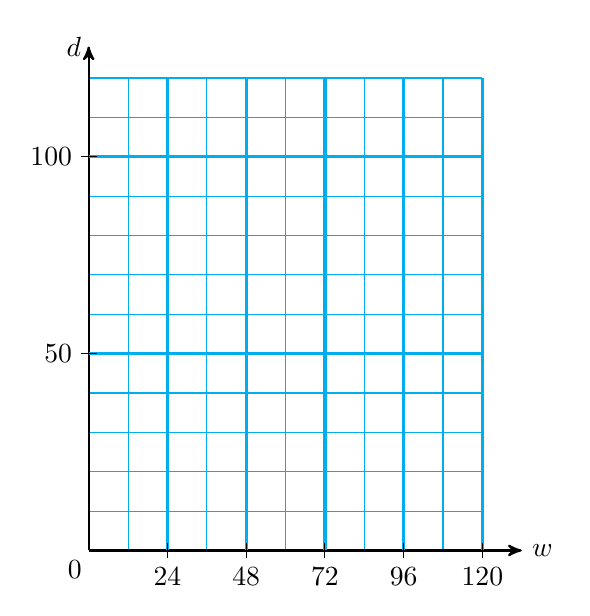
\begin{tikzpicture} [scale=.50]
\coordinate (O) at (0,0);
\draw[cyan] (O) grid (10,12);
\draw[black,thick, ->, >=stealth'] (O)--(11,0) node[right]{$w$};
\draw[black,thick, ->, >=stealth'] (O)--(0,12.8) node[left, xshift=1]{$d$};
\foreach \x [evaluate=\x as \xi using int( 12* \x )]in  {2,4,6,8,10} {
 \draw[cyan,very thick] (\x,0) --(\x,12); 
 \draw[black] (\x,.2) --++(0,-.4)  node[below, yshift=-2, fill=white, inner sep=1]   {$\xi$};
}
\foreach \x [evaluate=\x as \xi using int( 10* \x )] in  {5,10} {
 \draw[cyan, very thick] (0,\x) --(10,\x); 
 \draw[black] (.2,\x) --++(-.4,0)  node[left, xshift=-2, fill=white, inner sep=1]   {$\xi$};
}
\node[below left, xshift=1] at (O) {0};
\end{tikzpicture}
\newline


hp-2-3-11ans  grid

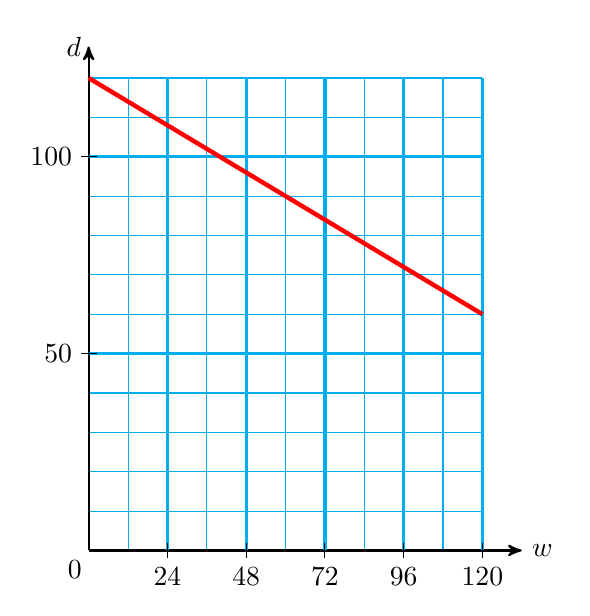
\begin{tikzpicture} [scale=.50]
\coordinate (O) at (0,0);
\draw[cyan] (O) grid (10,12);
\draw[black,thick, ->, >=stealth'] (O)--(11,0) node[right]{$w$};
\draw[black,thick, ->, >=stealth'] (O)--(0,12.8) node[left, xshift=1]{$d$};
\foreach \x [evaluate=\x as \xi using int( 12* \x )]in  {2,4,6,8,10} {
 \draw[cyan,very thick] (\x,0) --(\x,12); 
 \draw[black] (\x,.2) --++(0,-.4)  node[below, yshift=-2, fill=white, inner sep=1]   {$\xi$};
}
\foreach \x [evaluate=\x as \xi using int( 10* \x )] in  {5,10} {
 \draw[cyan, very thick] (0,\x) --(10,\x); 
 \draw[black] (.2,\x) --++(-.4,0)  node[left, xshift=-2, fill=white, inner sep=1]   {$\xi$};
}
\draw[red, ultra thick] (0,12)--(10,6);
\node[below left, xshift=1] at (O) {0};
\end{tikzpicture}
\newline


hp-2-3-12 10-by-10 grid

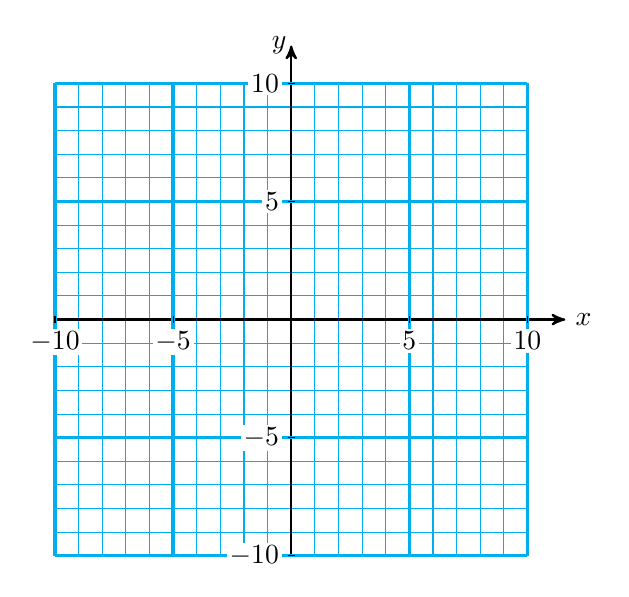
\begin{tikzpicture} [scale=.3]
\coordinate (O) at (0,0);
\draw[cyan] (-10,-10) grid (10,10);
\draw[black,thick, ->, >=stealth'] (-10,0)--(11.6,0) node[right]{$x$};
\draw[black,thick, ->, >=stealth'] (0,-10)--(0,11.6) node[left, xshift=2]{$y$};
\foreach \x in  {-5, 5, -10, 10} {
 \draw[cyan, very thick] (\x,-10) --++(0,20);
 \draw[cyan, very thick] (-10,\x) --++(20,0);
 \draw[black] (\x,.15) --++(0,-.3)  node[below, yshift=-2, fill=white, inner sep=1]   {$\x$};
 \draw[black] (.15,\x) --++(-.3,0)  node[left, xshift=-2, fill=white, inner sep=1]   {$\x$};
}
\end{tikzpicture}
\newline


hp-2-3-13ans 10-by-10 grid

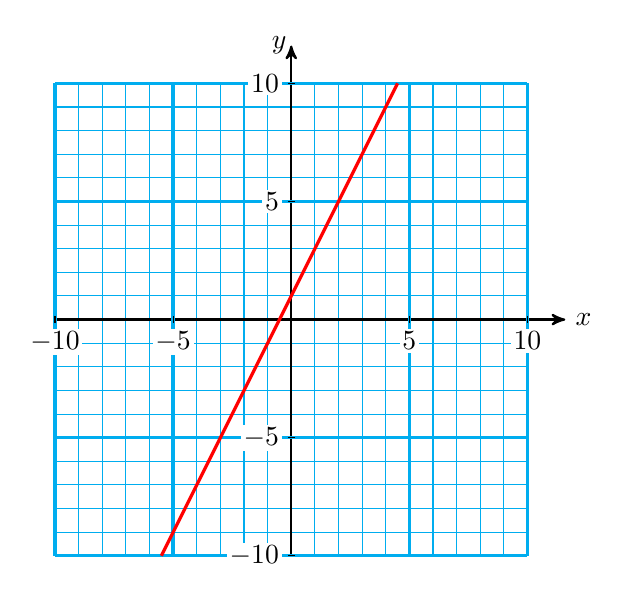
\begin{tikzpicture} [scale=.3]
\coordinate (O) at (0,0);
\draw[cyan] (-10,-10) grid (10,10);
\draw[black,thick, ->, >=stealth'] (-10,0)--(11.6,0) node[right]{$x$};
\draw[black,thick, ->, >=stealth'] (0,-10)--(0,11.6) node[left, xshift=2]{$y$};
\foreach \x in  {-5, 5, -10, 10} {
 \draw[cyan, very thick] (\x,-10) --++(0,20);
 \draw[cyan, very thick] (-10,\x) --++(20,0);
 \draw[black] (\x,.15) --++(0,-.3)  node[below, yshift=-2, fill=white, inner sep=1]   {$\x$};
 \draw[black] (.15,\x) --++(-.3,0)  node[left, xshift=-2, fill=white, inner sep=1]   {$\x$};
}
\draw[red,very thick] (-11/2,-10)--(9/2,10);
\end{tikzpicture}
\newline


hp-2-3-15ans 10-by-10 grid

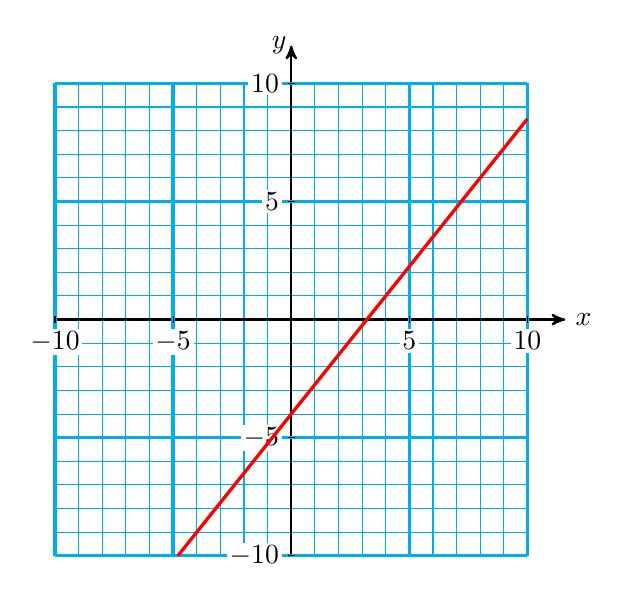
\begin{tikzpicture} [scale=.3]
\coordinate (O) at (0,0);
\draw[cyan] (-10,-10) grid (10,10);
\draw[black,thick, ->, >=stealth'] (-10,0)--(11.6,0) node[right]{$x$};
\draw[black,thick, ->, >=stealth'] (0,-10)--(0,11.6) node[left, xshift=2]{$y$};
\foreach \x in  {-5, 5, -10, 10} {
 \draw[cyan, very thick] (\x,-10) --++(0,20);
 \draw[cyan, very thick] (-10,\x) --++(20,0);
 \draw[black] (\x,.15) --++(0,-.3)  node[below, yshift=-2, fill=white, inner sep=1]   {$\x$};
 \draw[black] (.15,\x) --++(-.3,0)  node[left, xshift=-2, fill=white, inner sep=1]   {$\x$};
}
\draw[red,very thick] (-24/5,-10)--(10,34/4);
\end{tikzpicture}
\newline


hp-2-3-16 10-by-10 grid

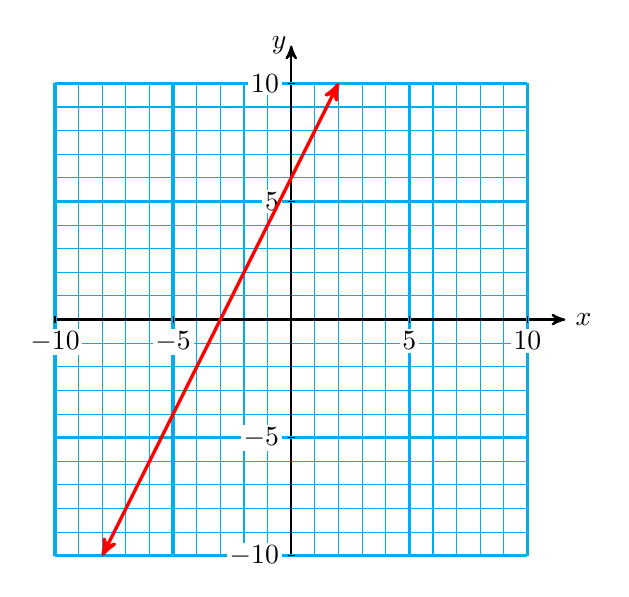
\begin{tikzpicture} [scale=.3]
\coordinate (O) at (0,0);
\draw[cyan] (-10,-10) grid (10,10);
\draw[black,thick, ->, >=stealth'] (-10,0)--(11.6,0) node[right]{$x$};
\draw[black,thick, ->, >=stealth'] (0,-10)--(0,11.6) node[left, xshift=2]{$y$};
\foreach \x in  {-5, 5, -10, 10} {
 \draw[cyan, very thick] (\x,-10) --++(0,20);
 \draw[cyan, very thick] (-10,\x) --++(20,0);
 \draw[black] (\x,.15) --++(0,-.3)  node[below, yshift=-2, fill=white, inner sep=1]   {$\x$};
 \draw[black] (.15,\x) --++(-.3,0)  node[left, xshift=-2, fill=white, inner sep=1]   {$\x$};
}
\draw[red,very thick, <->, >=stealth'] (-8,-10)--(2,10);
\end{tikzpicture}
\newline


hp-2-3-17 y=-9-x/4

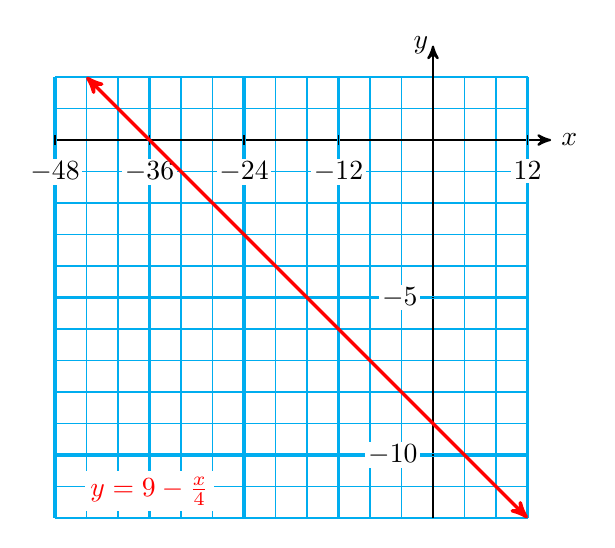
\begin{tikzpicture} [xscale=.1, yscale=.4]
\coordinate (O) at (0,0);
\draw[cyan] (-48,-12) grid[xstep=4] (12,2);
\draw[black,thick, ->, >=stealth'] (-48,0)--(15,0) node[right]{$x$};
\draw[black,thick, ->, >=stealth'] (0,-12)--(0,3) node[left, xshift=2]{$y$};
\foreach \x in  {-48,-36,-24,-12,12} {
 \draw[cyan, very thick] (\x,-12) --(\x,2);
 \draw[black] (\x,.15) --++(0,-.3)  node[below, yshift=-5, fill=white, inner sep=1]   {$\x$};
}
\foreach \x in  {-5,-10} {
 \draw[cyan, very thick] (-48,\x) --(12,\x);
 \draw[black] (.15,\x) --++(-.3,0)  node[left, xshift=-4, fill=white, inner sep=1]   {$\x$};
}
\draw[red,very thick, <->, >=stealth'] (-44,2)--(12,-12);
\node[below, text=red,fill=white, inner sep=2] at (-36,-10.5) {$y=9-\frac{x}{4}$};
\end{tikzpicture}
\newline


hp-2-3-18 y=7-2x/3

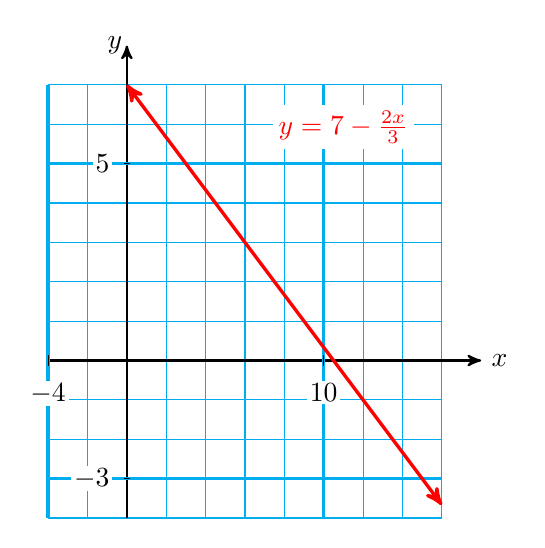
\begin{tikzpicture} [xscale=.25, yscale=.5]
\draw[cyan] (-4,-4) grid[xstep=2] (16,7);
\draw[black,thick, ->, >=stealth'] (-4,0)--(18,0) node[right]{$x$};
\draw[black,thick, ->, >=stealth'] (0,-4)--(0,8) node[left, xshift=2]{$y$};
\foreach \x in  {-4,10} {
 \draw[cyan, very thick] (\x,-4) --(\x,7);
 \draw[black] (\x,.15) --++(0,-.3)  node[below, yshift=-5, fill=white, inner sep=1]   {$\x$};
}
\foreach \x in  {-3,5} {
 \draw[cyan, very thick] (-4,\x) --(16,\x);
 \draw[black] (.15,\x) --++(-.3,0)  node[left, xshift=-4, fill=white, inner sep=1]   {$\x$};
}
\draw[red,very thick, <->, >=stealth'] (0,7)--(16,{7-32/3});
\node[below, text=red,fill=white, inner sep=2] at (11,6.5) {$y=7-\frac{2x}{3}$};
\end{tikzpicture}
\newline


hp-2-3-19 y=7-2x/337.21-8.4t

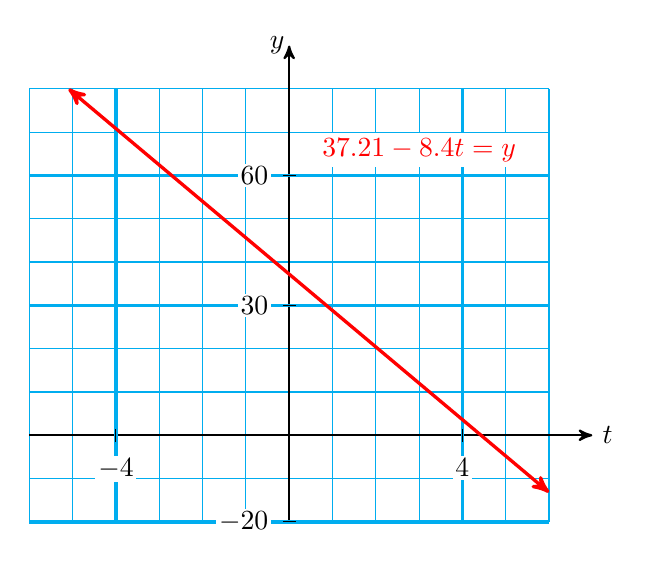
\begin{tikzpicture} [xscale=.55, yscale=.055]
\draw[cyan] (-6,-20) grid[ystep=10] (6,80);
\draw[black,thick, ->, >=stealth'] (-6,0)--(7,0) node[right]{$t$};
\draw[black,thick, ->, >=stealth'] (0,-20)--(0,90) node[left, xshift=2]{$y$};
\foreach \x in  {-4,4} {
 \draw[cyan, very thick] (\x,-20) --(\x,80);
 \draw[black] (\x,1.5) --++(0,-3)  node[below, yshift=-5, fill=white, inner sep=1]   {$\x$};
}
\foreach \x in  {-20,30,60} {
 \draw[cyan, very thick] (-6,\x) --(6,\x);
 \draw[black] (.15,\x) --++(-.3,0)  node[left, xshift=-4, fill=white, inner sep=1]   {$\x$};
}
\draw[red,very thick, <->, >=stealth'] ({(80-37.21)/(-8.4)},80)--(6,{37.21-8.4*6});
\node[below, text=red,fill=white, inner sep=2] at (3,70) {$37.21-8.4t=y$};
\end{tikzpicture}
\newline


hp-2-3-19 y=-3.65+0.1x

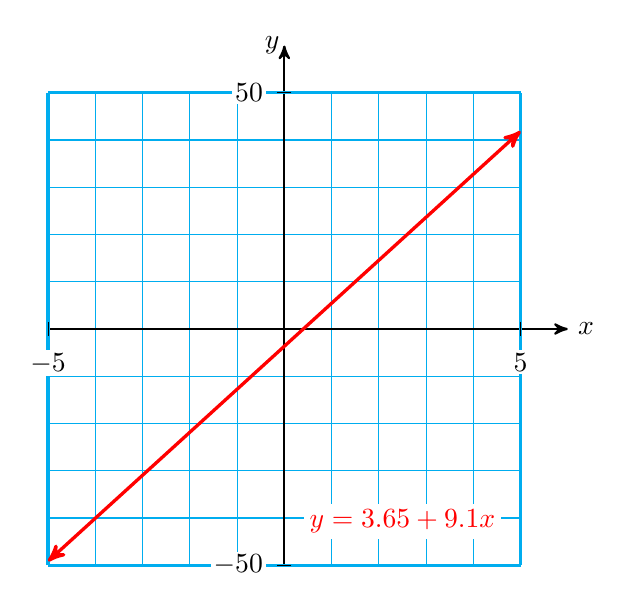
\begin{tikzpicture} [xscale=.6, yscale=.06]
\draw[cyan] (-5,-50) grid[ystep=10] (5,50);
\draw[black,thick, ->, >=stealth'] (-5,0)--(6,0) node[right]{$x$};
\draw[black,thick, ->, >=stealth'] (0,-50)--(0,60) node[left, xshift=2]{$y$};
\foreach \x in  {-5,5} {
 \draw[cyan, very thick] (\x,-50) --(\x,50);
 \draw[black] (\x,1.5) --++(0,-3)  node[below, yshift=-5, fill=white, inner sep=1]   {$\x$};
}
\foreach \x in  {-50,50} {
 \draw[cyan, very thick] (-5,\x) --(5,\x);
 \draw[black] (.15,\x) --++(-.3,0)  node[left, xshift=-4, fill=white, inner sep=1]   {$\x$};
}
\draw[red,very thick, <->, >=stealth'] (5,{-3.65+9.1*5})--(-5,{-3.65+9.1*-5});
\node[below, text=red,fill=white, inner sep=2] at (2.5,-37) {$y=3.65+9.1x$};
\end{tikzpicture}
\newline



\section{Chap 2 Section 4}



fig-2-4-ex3

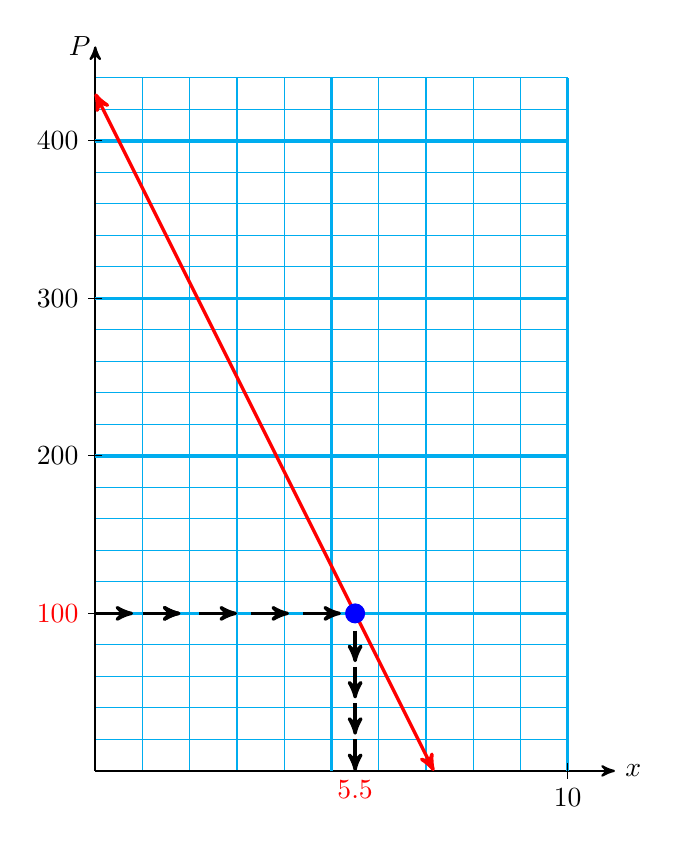
\begin{tikzpicture} [xscale=.6, yscale=.02]
\coordinate (O) at (0,0);
\draw[cyan] (O) grid[ystep=20] (10,440);
\draw[black,thick, ->, >=stealth'] (O)--(11,0) node[right]{$x$};
\draw[black,thick, ->, >=stealth'] (O)--(0,460) node[left, xshift=2]{$P$};
\foreach \x in  {10} {
 \draw[cyan, very thick] (\x,0) --(\x,440);
 \draw[black] (\x,5) --++(0,-10)  node[below] {$\x$};
}
\draw[cyan, very thick] (5,0) --(5,440);
\foreach \x in  {200, 300, 400} {
 \draw[cyan, very thick] (0,\x) --(10,\x);
 \draw[black] (.15,\x) --++(-.3,0)  node[left] {$\x$};
}
\draw[cyan, thick] (0,100) --(10,100);
\draw[red,very thick, <->, >=stealth'] (0,430)--({43/6},0);
\node[below, text=red] at (5.5,0) {$5.5$};
\draw[black] (.15,100)--++(-.3,0) node[left, text=red] {$100$};
\filldraw[blue] (5.5,100) ellipse (.2cm and 6cm);
\foreach \x in {0,1,1,2.2,3.3,4.4}{
 \draw[black, very thick, ->,>=stealth'] (\x,100)--++(.8,0);
 }
\foreach \x in {89, 66, 43, 20}{
 \draw[black, very thick, ->,>=stealth'] (5.5, \x)--++(0, -20);
 }
\end{tikzpicture}
\newline

fig-2-4-ex4 number line

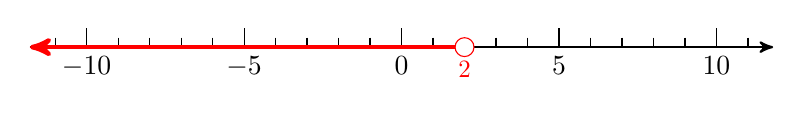
\begin{tikzpicture} [scale=.4]
\draw[black,thick, ->, >=stealth'] (-11.8,0)--(11.8,0);
\foreach \x in  {-11, -10, ..., 11} {
 \draw[black] (\x,.3) --++(0,-.3);
}
\foreach \x in  {-10,-5,0,5,10} {
 \draw[black] (\x,.6) --++(0,-.6)  node[below] {$\x$};
}
\draw[red, ultra thick, ->, >=stealth'] (2,0)--(-11.8,0);
\draw[red, fill=white] (2,0) circle (3mm);
\node[below, yshift=-2, text=red, scale=.9] at (2,0) {$2$};
\end{tikzpicture}
\newline

fig-2-4-1 number line

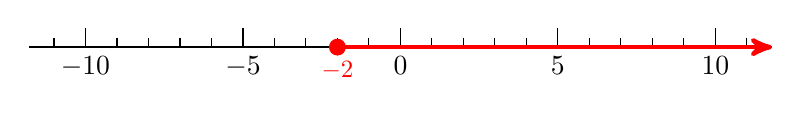
\begin{tikzpicture} [scale=.4]
\draw[black,thick, ->, >=stealth'] (-11.8,0)--(11.8,0);
\foreach \x in  {-11, -10, ..., 11} {
 \draw[black] (\x,.3) --++(0,-.3);
}
\foreach \x in  {-10,-5,0,5,10} {
 \draw[black] (\x,.6) --++(0,-.6)  node[below] {$\x$};
}
\draw[red, ultra thick, ->, >=stealth'] (-2,0)--(11.8,0);
\draw[red, fill=red] (-2,0) circle (2.5mm);
\node[below, yshift=-2, text=red, scale=.9] at (-2,0) {$-2$};
\end{tikzpicture}
\newline

fig-2-4-ex5 number line

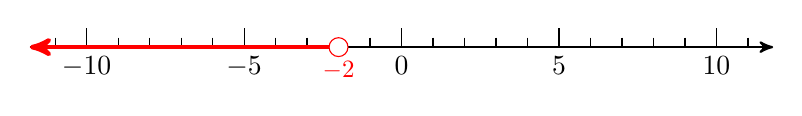
\begin{tikzpicture} [scale=.4]
\draw[black,thick, ->, >=stealth'] (-11.8,0)--(11.8,0);
\foreach \x in  {-11, -10, ..., 11} {
 \draw[black] (\x,.3) --++(0,-.3);
}
\foreach \x in  {-10,-5,0,5,10} {
 \draw[black] (\x,.6) --++(0,-.6)  node[below] {$\x$};
}
\draw[red, ultra thick, ->, >=stealth'] (-2,0)--(-11.8,0);
\draw[red, fill=white] (-2,0) circle (3mm);
\node[below, yshift=-2, text=red, scale=.9] at (-2,0) {$-2$};
\end{tikzpicture}
\newline

fig-2-4-ex5 number line

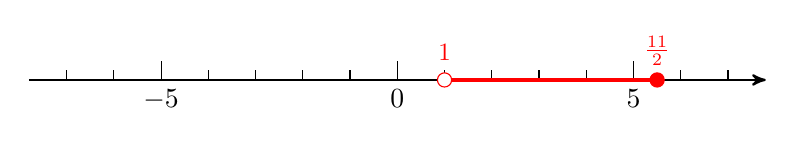
\begin{tikzpicture} [scale=.6]
\draw[black,thick, ->, >=stealth'] (-7.8,0)--(7.8,0);
\foreach \x in  {-7, -6, ..., 7} {
 \draw[black] (\x,.2) --++(0,-.2);
}
\foreach \x in  {-5,0,5} {
 \draw[black] (\x,.4) --++(0,-.4)  node[below] {$\x$};
}
\draw[red, ultra thick] (1,0)--(11/2,0);
\draw[red, fill=white] (1,0) circle (1.5mm);
\node[above, yshift=4, text=red, scale=.9] at (1,0) {$1$};
\draw[red, fill=red] (11/2,0) circle (1.5mm);
\node[above, yshift=2, text=red, scale=.9] at (11/2,0) {$\frac{11}{2}$};
\end{tikzpicture}
\newline

hp2-4-21ans number line

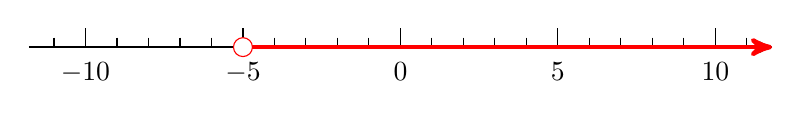
\begin{tikzpicture} [scale=.4]
\draw[black,thick, ->, >=stealth'] (-11.8,0)--(11.8,0);
\foreach \x in  {-11, -10, ..., 11} {
 \draw[black] (\x,.3) --++(0,-.3);
}
\foreach \x in  {-10,-5,0,5,10} {
 \draw[black] (\x,.6) --++(0,-.6)  node[below,, yshift=-2] {$\x$};
}
\draw[red, ultra thick, ->, >=stealth'] (-5,0)--(11.8,0);
\draw[red, fill=white] (-5,0) circle (3mm);
\end{tikzpicture}
\newline

hp2-4-23ans number line

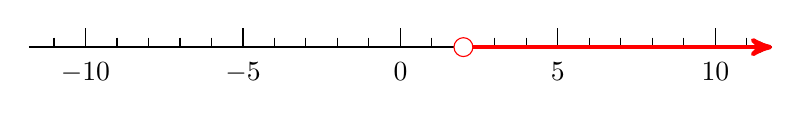
\begin{tikzpicture} [scale=.4]
\draw[black,thick, ->, >=stealth'] (-11.8,0)--(11.8,0);
\foreach \x in  {-11, -10, ..., 11} {
 \draw[black] (\x,.3) --++(0,-.3);
}
\foreach \x in  {-10,-5,0,5,10} {
 \draw[black] (\x,.6) --++(0,-.6)  node[below,, yshift=-2] {$\x$};
}
\draw[red, ultra thick, ->, >=stealth'] (2,0)--(11.8,0);
\draw[red, fill=white] (2,0) circle (3mm);
\end{tikzpicture}
\newline

hp2-4-25ans number line

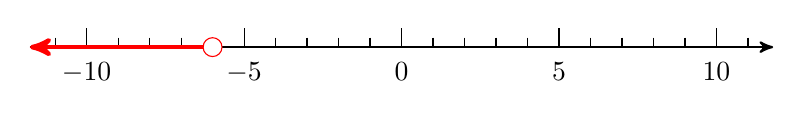
\begin{tikzpicture} [scale=.4]
\draw[black,thick, ->, >=stealth'] (-11.8,0)--(11.8,0);
\foreach \x in  {-11, -10, ..., 11} {
 \draw[black] (\x,.3) --++(0,-.3);
}
\foreach \x in  {-10,-5,0,5,10} {
 \draw[black] (\x,.6) --++(0,-.6)  node[below,, yshift=-2] {$\x$};
}
\draw[red, ultra thick, ->, >=stealth'] (-6,0)--(-11.8,0);
\draw[red, fill=white] (-6,0) circle (3mm);
\end{tikzpicture}
\newline

hp2-4-27ans number line

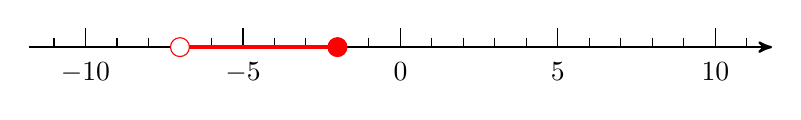
\begin{tikzpicture} [scale=.4]
\draw[black,thick, ->, >=stealth'] (-11.8,0)--(11.8,0);
\foreach \x in  {-11, -10, ..., 11} {
 \draw[black] (\x,.3) --++(0,-.3);
}
\foreach \x in  {-10,-5,0,5,10} {
 \draw[black] (\x,.6) --++(0,-.6)  node[below,, yshift=-2] {$\x$};
}
\draw[red, ultra thick] (-7,0)--(-2,0);
\draw[red, fill=white] (-7,0) circle (3mm);
\draw[red, fill=red] (-2,0) circle (3mm);
\end{tikzpicture}
\newline


hp-2-4-32

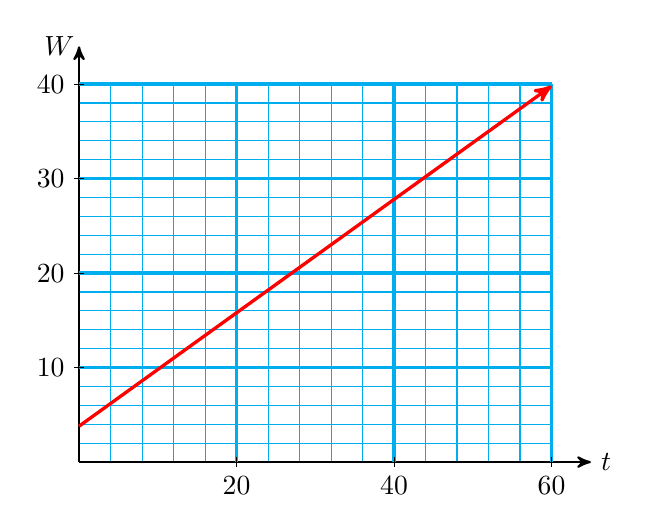
\begin{tikzpicture} [xscale=.1, yscale=.12]
\coordinate (O) at (0,0);
\draw[cyan] (O) grid[xstep=4, ystep=2] (60,40);
\draw[black,thick, ->, >=stealth'] (O)--(65,0) node[right]{$t$};
\draw[black,thick, ->, >=stealth'] (O)--(0,44) node[left, xshift=2]{$W$};
\foreach \x in  {20,40,60} {
 \draw[cyan, very thick] (\x,0) --(\x,40);
 \draw[black] (\x,.5) --++(0,-1)  node[below]   {$\x$};
}
\foreach \x in  {10,20,30,40} {
 \draw[cyan, very thick] (0,\x) --(60,\x);
 \draw[black] (.6,\x) --++(-1.2,0)  node[left]   {$\x$};
}
\draw[red,very thick, ->, >=stealth'] (0,3.8)--(60,{3.8+60*0.6});
\end{tikzpicture}
\newline


hp-2-4-33

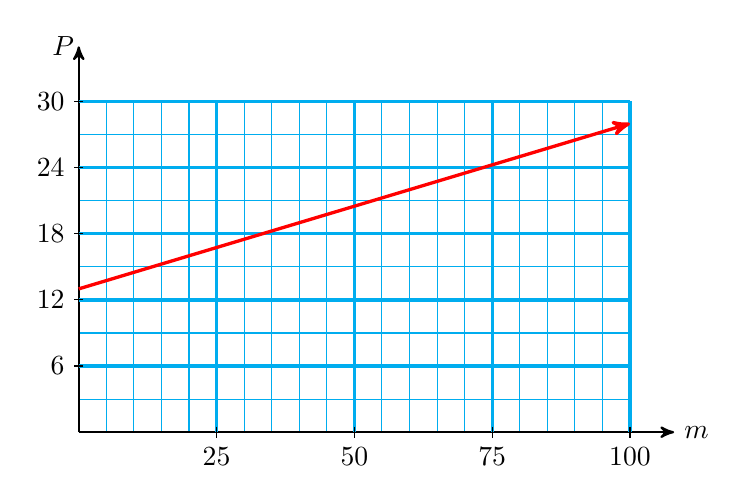
\begin{tikzpicture} [xscale=.07, yscale=.14]
\coordinate (O) at (0,0);
\draw[cyan] (O) grid[xstep=5, ystep=3] (100,30);
\draw[black,thick, ->, >=stealth'] (O)--(108,0) node[right]{$m$};
\draw[black,thick, ->, >=stealth'] (O)--(0,35) node[left, xshift=2]{$P$};
\foreach \x in  {25,50,75,100} {
 \draw[cyan, very thick] (\x,0) --(\x,30);
 \draw[black] (\x,.5) --++(0,-1)  node[below]   {$\x$};
}
\foreach \x in  {6,12,18,24,30} {
 \draw[cyan, very thick] (0,\x) --(100,\x);
 \draw[black] (.8,\x) --++(-1.6,0)  node[left]   {$\x$};
}
\draw[red,very thick, ->, >=stealth'] (0,13)--(100,{13+100*0.15});
\end{tikzpicture}
\newline


hp-2-4-41 rectangles

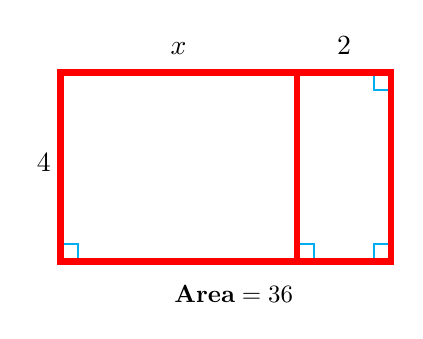
\begin{tikzpicture} 
\coordinate(O) at (0,0);
\coordinate(A) at (4.2,2.4);
\coordinate(B) at (3.,0);
\draw[cyan,thick] (O) rectangle ++(.22,.22);
\draw[cyan,thick] (B) rectangle ++(.22,.22);
\draw[cyan,thick] (A) rectangle ++(-.22,-.22);
\draw[cyan,thick] (4.2,0) rectangle ++(-.22,.22);
\draw[red, line width=.8mm] (B) --++(0,2.4);
\draw[red, line width=.8mm] (O) rectangle (A);
\node[below, scale=.9] at (2.2,-.2) {$\textbf{Area}=36$};
\node[left] at (0,1.25) {$4$};
\node[above] at (1.5,2.5) {$x$};
\node[above] at (3.6,2.5) {$2$};
\end{tikzpicture}
\newline


hp-2-4-42 triangle

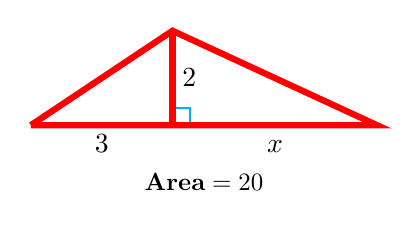
\begin{tikzpicture} 
\coordinate(O) at (0,0);
\coordinate(A) at (4.4,0);
\coordinate(B) at (1.8,1.2);
\coordinate(C) at (1.8,0);
\draw[cyan,thick] (C) rectangle ++(.22,.22);
\draw[red,line width=.8mm] (O)--(A)--(B)--(O);
\draw[red,line width=.8mm] (B)--(C);
\node[right] at (1.8,0.6) {$2$};
\node[below] at (.9,0) {$3$};
\node[below, yshift=-2] at (3.1,0,0) {$x$};
\node[below, scale=.9] at (2.2,-.5) {$\textbf{Area}=20$};
\end{tikzpicture}
\newline



\section{Chap 2 Section 4}




fig-2-5-ex7

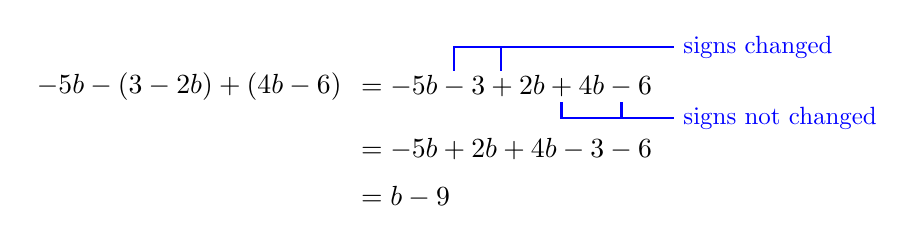
\begin{tikzpicture} 
\coordinate (O) at (0,0);
\node[left] at (O) {$-5b-(3-2b)+(4b-6)$};
\node[right] at (O) {$=-5b-3+2b +4b-6$};
\coordinate(A) at (1.3,0.2);
\draw[blue,thick] (A) --++(0,.3)--++(2.8,0) node[right, scale=.9] {signs changed};
\coordinate(B) at (1.9,0.2);
\draw[blue,thick] (B) --++(0,.3);
\coordinate(C) at (2.67,-0.2);
\draw[blue,thick] (C) --++(0,-.2)--++(1.43,0) node[right, scale=.9] {signs not changed};
\coordinate(D) at (3.43,-0.2);
\draw[blue,thick] (D) --++(0,-.2);
\coordinate (O2) at (0,-0.8);
\node[right] at (O2) {$=-5b+2b +4b-3-6$};
\coordinate (O3) at (0,-1.4);
\node[right] at (O3) {$=b-9$};
\end{tikzpicture}
\newline


hp-2-5-23 rectangle

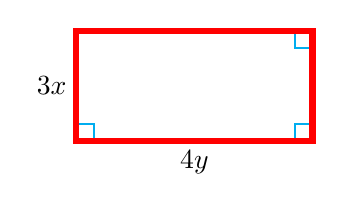
\begin{tikzpicture} 
\coordinate(O) at (0,0);
\coordinate(A) at (3,1.4);
\draw[cyan,thick] (O) rectangle ++(.22,.22);
\draw[cyan,thick] (3,0) rectangle ++(-.22,.22);
\draw[cyan,thick] (A) rectangle ++(-.22,-.22);
\draw[red, line width=.8mm] (O) rectangle (A);
\node[below] at (1.5,0) {$4y$};
\node[left] at (0,0.7) {$3x$};
\end{tikzpicture}
\newline


hp-2-5-24 trapezoid

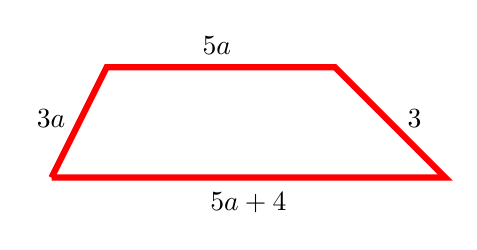
\begin{tikzpicture} 
\coordinate(O) at (0,0);
\coordinate(A) at (5,0);
\coordinate(B) at (3.6,1.4);
\coordinate(C) at (.7,1.4);
\draw[red,line width=.8mm] (O)--(A)--(B)--(C)--(O);
\node[left] at (0.3,0.75) {$3a$};
\node[right] at (4.4,0.75) {$3$};
\node[above, yshift=1] at (2.1,1.4) {$5a$};
\node[below, yshift=-2] at (2.5,0) {$5a+4$};
\end{tikzpicture}
\newline




\section{Chap 2 Review}


cr2-11  grid

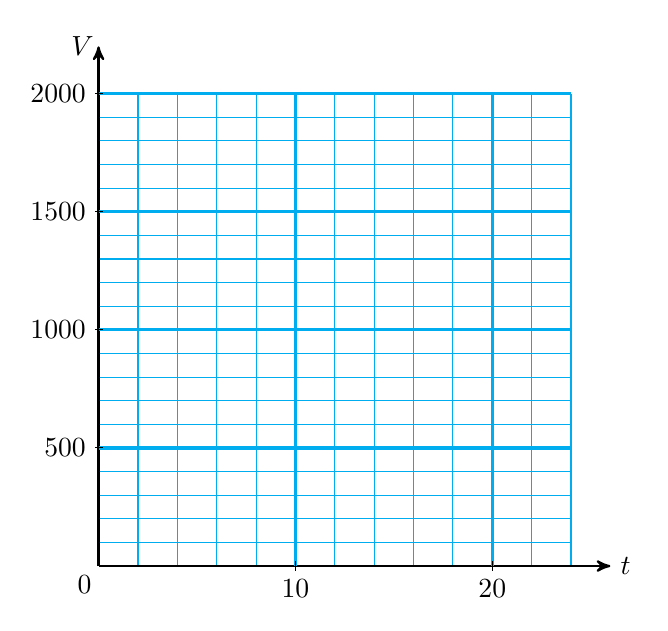
\begin{tikzpicture} [xscale=.25, yscale=0.3]
\coordinate (O) at (0,0);
\draw[cyan] (O) grid[xstep=2] (24,20);
\draw[black,thick, ->, >=stealth'] (O)--(26,0) node[right]{$t$};
\draw[black,thick, ->, >=stealth'] (O)--(0,22) node[left, xshift=2]{$V$};
\foreach \x in  {10, 20} {
 \draw[cyan,very thick] (\x,0) --(\x,20); 
 \draw[black] (\x,.2) --++(0,-.4)  node[below, yshift=-2, fill=white, inner sep=1]   {$\x$};
}
\foreach \x [evaluate=\x as \xi using int( 100* \x )] in  {5,10,15,20} {
 \draw[cyan, very thick] (0,\x) --(24,\x); 
 \draw[black] (.2,\x) --++(-.4,0)  node[left, xshift=-2, fill=white, inner sep=1]   {$\xi$};
}
\node[below left, xshift=1] at (O) {0};
\end{tikzpicture}
\newline


cr2-11ans

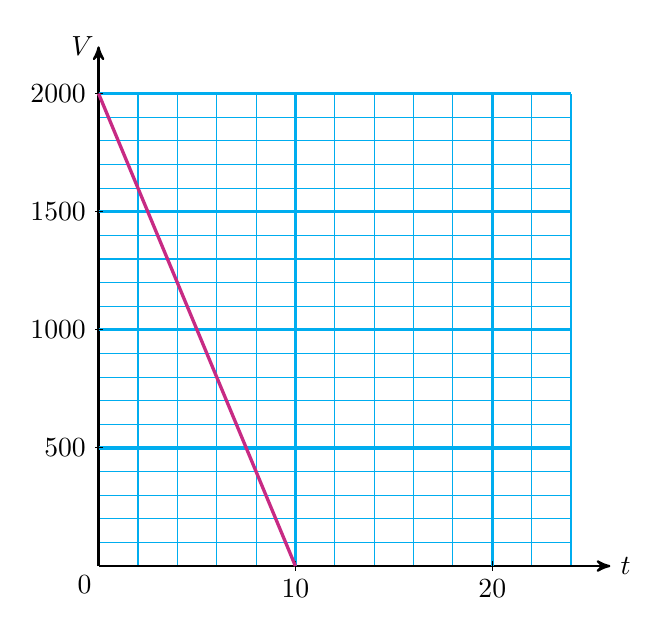
\begin{tikzpicture} [xscale=.25, yscale=0.3]
\coordinate (O) at (0,0);
\draw[cyan] (O) grid[xstep=2] (24,20);
\draw[black,thick, ->, >=stealth'] (O)--(26,0) node[right]{$t$};
\draw[black,thick, ->, >=stealth'] (O)--(0,22) node[left, xshift=2]{$V$};
\foreach \x in  {10, 20} {
 \draw[cyan,very thick] (\x,0) --(\x,20); 
 \draw[black] (\x,.2) --++(0,-.4)  node[below, yshift=-2, fill=white, inner sep=1]   {$\x$};
}
\foreach \x [evaluate=\x as \xi using int( 100* \x )] in  {5,10,15,20} {
 \draw[cyan, very thick] (0,\x) --(24,\x); 
 \draw[black] (.2,\x) --++(-.4,0)  node[left, xshift=-2, fill=white, inner sep=1]   {$\xi$};
}
\node[below left, xshift=1] at (O) {0};
\draw[magenta!80!black, very thick] (0,20)--(10,0);
\end{tikzpicture}
\newline


cr2-12  grid

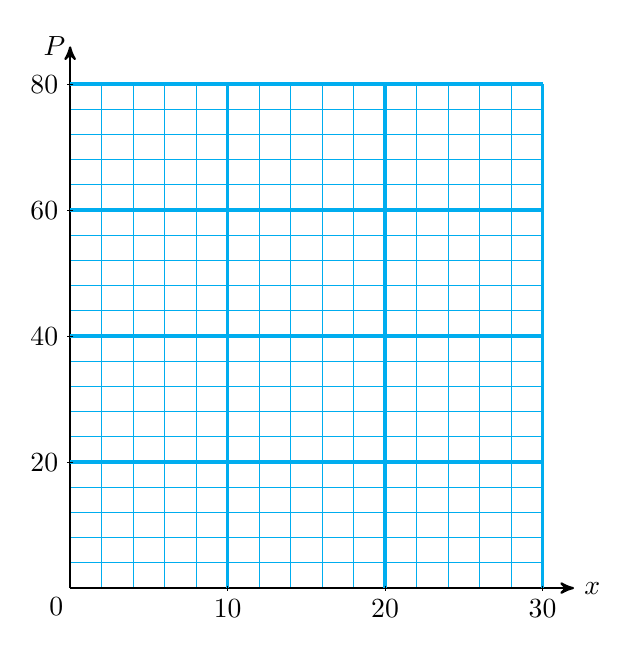
\begin{tikzpicture} [xscale=.2, yscale=0.08]
\coordinate (O) at (0,0);
\draw[cyan] (O) grid[xstep=2, ystep=4] (30,80);
\draw[black,thick, ->, >=stealth'] (O)--(32,0) node[right]{$x$};
\draw[black,thick, ->, >=stealth'] (O)--(0,86) node[left, xshift=2]{$P$};
\foreach \x in  {10, 20,30} {
 \draw[cyan,very thick] (\x,0) --(\x,80); 
 \draw[black] (\x,.4) --++(0,-.8)  node[below, yshift=-2, fill=white, inner sep=1]   {$\x$};
}
\foreach \x in {20,40,60,80} {
 \draw[cyan, very thick] (0,\x) --(30,\x); 
 \draw[black] (.2,\x) --++(-.4,0)  node[left, xshift=-2, fill=white, inner sep=1]   {$\x$};
}
\node[below left, xshift=1] at (O) {0};
\end{tikzpicture}
\newline


cr2-43  grid

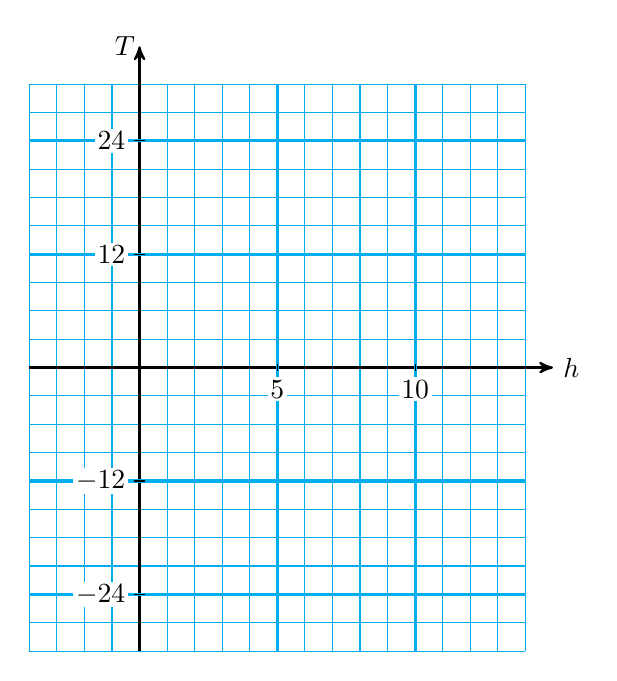
\begin{tikzpicture} [xscale=.35, yscale=0.12]
\draw[cyan] (-4,-30) grid[ ystep=3] (14,30);
\draw[black,thick, ->, >=stealth'] (-4,0)--(15,0) node[right]{$h$};
\draw[black,thick, ->, >=stealth'] (0,-30)--(0,34) node[left, xshift=2]{$T$};
\foreach \x in  {5, 10} {
 \draw[cyan,very thick] (\x,-30) --(\x,30); 
 \draw[black] (\x,.4) --++(0,-.8)  node[below, yshift=-2, fill=white, inner sep=1]   {$\x$};
}
\foreach \x in {-24,-12,12,24} {
 \draw[cyan, very thick] (-4,\x) --(14,\x); 
 \draw[black] (.2,\x) --++(-.4,0)  node[left, xshift=-2, fill=white, inner sep=1]   {$\x$};
}
\end{tikzpicture}
\newline


cr2-45ans

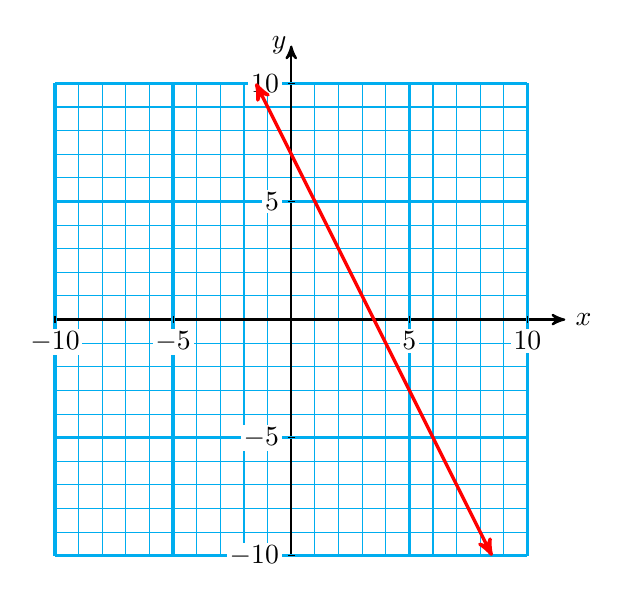
\begin{tikzpicture} [scale=.3]
\coordinate (O) at (0,0);
\draw[cyan] (-10,-10) grid (10,10);
\draw[black,thick, ->, >=stealth'] (-10,0)--(11.6,0) node[right]{$x$};
\draw[black,thick, ->, >=stealth'] (0,-10)--(0,11.6) node[left, xshift=2]{$y$};
\foreach \x in  {-5, 5, -10, 10} {
 \draw[cyan, very thick] (\x,-10) --++(0,20);
 \draw[cyan, very thick] (-10,\x) --++(20,0);
 \draw[black] (\x,.15) --++(0,-.3)  node[below, yshift=-2, fill=white, inner sep=1]   {$\x$};
 \draw[black] (.15,\x) --++(-.3,0)  node[left, xshift=-2, fill=white, inner sep=1]   {$\x$};
}
\draw[red,very thick, <->, >=stealth'] (-1.5,10)--(8.5,-10);
\end{tikzpicture}
\newline


cr2-43ans

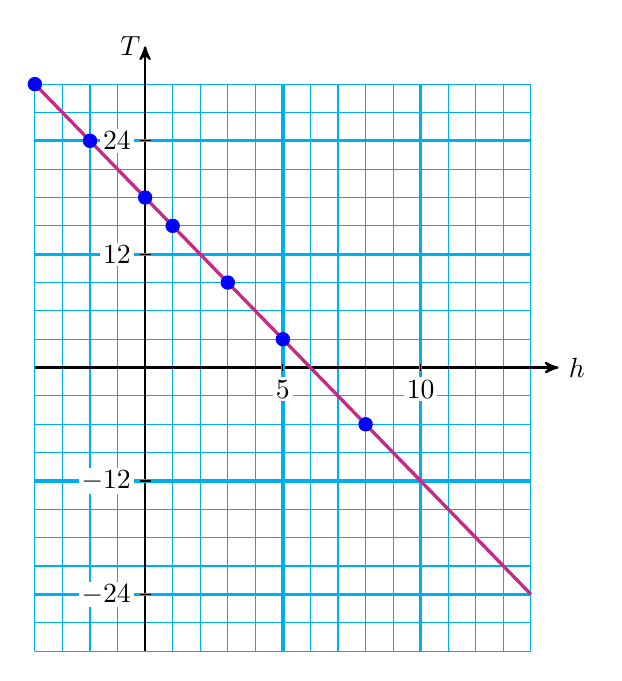
\begin{tikzpicture} [xscale=.35, yscale=0.12]
\draw[cyan] (-4,-30) grid[ ystep=3] (14,30);
\draw[black,thick, ->, >=stealth'] (-4,0)--(15,0) node[right]{$h$};
\draw[black,thick, ->, >=stealth'] (0,-30)--(0,34) node[left, xshift=2]{$T$};
\foreach \x in  {5, 10} {
 \draw[cyan,very thick] (\x,-30) --(\x,30); 
 \draw[black] (\x,.4) --++(0,-.8)  node[below, yshift=-2, fill=white, inner sep=1]   {$\x$};
}
\foreach \x in {-24,-12,12,24} {
 \draw[cyan, very thick] (-4,\x) --(14,\x); 
 \draw[black] (.2,\x) --++(-.4,0)  node[left, xshift=-2, fill=white, inner sep=1]   {$\x$};
}
\draw[magenta!80!black, very thick] (-4,30) -- (14,-24);
\foreach \x in {-4,-2,0,1,3,5,8} {
 \filldraw[blue] ((\x,{18-3*\x}) ellipse (2.41mm and 7mm);
}
\end{tikzpicture}
\newline


cr2-55  grid

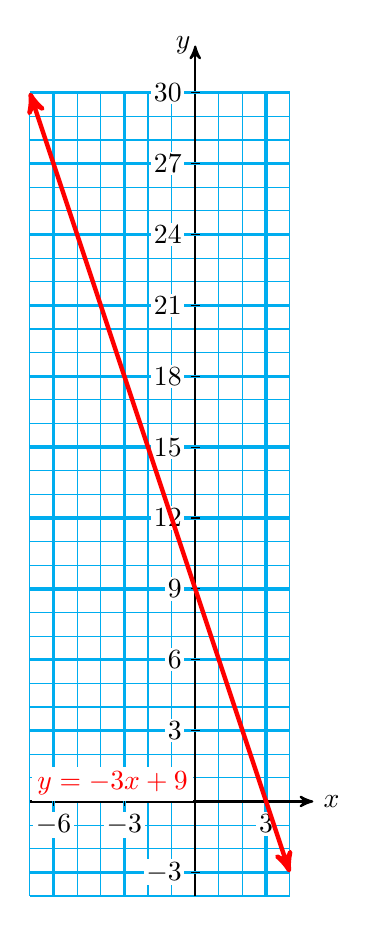
\begin{tikzpicture} [scale=0.3]
\draw[cyan] (-7,-4) grid (4,30);
\draw[black,thick, ->, >=stealth'] (-7,0)--(5,0) node[right]{$x$};
\draw[black,thick, ->, >=stealth'] (0,-4)--(0,32) node[left, xshift=2]{$y$};
\foreach \x in  {-6,-3,3} {
 \draw[cyan,very thick] (\x,-4) --(\x,30); 
 \draw[black] (\x,.2) --++(0,-.4)  node[below, yshift=-2, fill=white, inner sep=1]   {$\x$};
}
\foreach \x in {-3,3,6,9,12,15,18,21,24,27,30} {
 \draw[cyan, very thick] (-7,\x) --(4,\x); 
 \draw[black] (.2,\x) --++(-.4,0)  node[left, xshift=-2, fill=white, inner sep=1]   {$\x$};
}
\draw[red, ultra thick, <->, >=stealth'] (-7,30)--(4,-3);
\node[above, text=red, fill=white, inner sep=2] at (-3.5,0) {$y=-3x+9$};
\end{tikzpicture}
\newline


cr2-56  grid

\begin{tikzpicture} [scale=0.3]
\draw[cyan] (-6,-20) grid (12,5);
\draw[black,thick, ->, >=stealth'] (-6,0)--(13,0) node[right]{$x$};
\draw[black,thick, ->, >=stealth'] (0,-20)--(0,6.5) node[left, xshift=2]{$y$};
\foreach \x [evaluate=\x as \xi using int( 10* \x )] in {-5,5,10} {
 \draw[cyan,very thick] (\x,-20) --(\x,5); 
 \draw[black] (\x,.2) --++(0,-.4)  node[below, yshift=-2, fill=white, inner sep=1]   {$\xi$};
}
\foreach \x [evaluate=\x as \xi using int( 200* \x )] in {-20,-15,-10,-5,5} {
 \draw[cyan, very thick] (-6,\x) --(12,\x); 
 \draw[black] (.2,\x) --++(-.4,0)  node[left, xshift=-2, fill=white, inner sep=1]   {$\xi$};
}
\draw[red, ultra thick, <->, >=stealth'] (-6,{(24*(-60)-1800)/200})--({280/24}, 5);
\node[above, text=red, fill=white, inner sep=2] at (7.2,-19.4) {$y=24x-1800$};
\end{tikzpicture}
\newline

cr2-59ans number line

\begin{tikzpicture} [scale=.4]
\draw[black,thick, ->, >=stealth'] (-7.8,0)--(7.8,0);
\foreach \x in  {-7,-6, ..., 7} {
 \draw[black] (\x,.3) --++(0,-.3);
}
\foreach \x in  {-5,0,5} {
 \draw[black] (\x,.6) --++(0,-.6)  node[below,, yshift=-2] {$\x$};
}
\draw[red, ultra thick, ->, >=stealth'] (3,0)--(7.8,0);
\draw[red, fill=red] (3,0) circle (3mm);
\node[left] at (-8.5,0) {$z \ge 3$};
\end{tikzpicture}
\newline

cr2-61ans number line

\begin{tikzpicture} [scale=.4]
\draw[black,thick, ->, >=stealth'] (-7.8,0)--(7.8,0);
\foreach \x in  {-7,-6, ..., 7} {
 \draw[black] (\x,.3) --++(0,-.3);
}
\foreach \x in  {-5,0,5} {
 \draw[black] (\x,.6) --++(0,-.6)  node[below,, yshift=-2] {$\x$};
}
\draw[red, ultra thick, ->, >=stealth'] (-5,0)--(7.8,0);
\draw[red, fill=white] (-5,0) circle (3mm);
\node[left] at (-8.5,0) {$k > -6$};
\end{tikzpicture}
\newline

cr2-63ans number line

\begin{tikzpicture} [scale=.4]
\draw[black,thick, ->, >=stealth'] (-2.8,0)--(11.8,0);
\foreach \x in  {-2,-1, ..., 11} {
 \draw[black] (\x,.3) --++(0,-.3);
}
\foreach \x in  {10,0,5} {
 \draw[black] (\x,.6) --++(0,-.6)  node[below,, yshift=-2] {$\x$};
}
\draw[red, ultra thick] (3,0)--(7,0);
\draw[red, fill=white] (7,0) circle (3mm);
\draw[red, fill=red] (3,0) circle (3mm);
\node[left] at (-3.5,0) {$7 > n \ge 3$};
\end{tikzpicture}
\newline





\end{document}
